% Heat-conduction lab report. Build from ../ with `make`.
% Rules: ../../report-rules.md (general), ../report-rules.md (heat conduction).
% Limits: 12 pages excluding cover + appendices (user, 2026-11-05); 16 numbered formulas INCLUDING theory (1)-(5) (user, 2026-11-05).
% Preamble copied from ../../freefall/report/main.tex (2026-11-04).
\documentclass[10pt,a4paper]{article}

\usepackage[a4paper,margin=2cm]{geometry}
\usepackage{amsmath}
\usepackage{graphicx}
\usepackage{float}  % [H]: figures and tables stay where they are written (user, 2026-10-30)
\usepackage{tikz}
\usepackage{xcolor}
\usepackage[labelsep=colon,font=small]{caption}
\usepackage{fontspec}
% LuaLaTeX + babel instead of XeLaTeX + polyglossia (2026-10-28): under XeTeX's bidi,
% \textcolor leaked to whole RTL lines; luacolor colours per character.
\usepackage{luacolor}
\usepackage[bidi=basic, layout=lists.tabular, main=hebrew, english]{babel}
% Times New Roman (macOS system font, has Hebrew). Frank Ruehl CLM's digits read as bold.
\babelfont[hebrew]{rm}{Times New Roman}
\newcommand{\textenglish}[1]{\foreignlanguage{english}{#1}}
% Second-level list labels (א), (ב)... In running text a sub-item is referred to as 1א (user, 2026-10-30).
\renewcommand{\theenumii}{\localecounter{letters}{enumii}}
\renewcommand{\labelenumii}{(\theenumii)}

% Paragraphs: no first-line indent, small gap between paragraphs (Word-like, as in the guide).
\setlength{\parindent}{0pt}
\setlength{\parskip}{4pt plus 1pt}

% Review colours: blue = text written by Claude, until the user approves it (no Doc in this
% report). Off for submission: \reviewfalse turns it black, the macro stays in the source.
\newif\ifreview \reviewtrue
\ifreview
  \colorlet{addedblue}{blue}
\else
  \colorlet{addedblue}{black}
\fi
\newcommand{\added}[1]{\textcolor{addedblue}{#1}}

% Visible placeholder for anything not written yet. Must not survive into the submitted PDF.
\newcommand{\TODO}[1]{\textcolor{red}{[#1]}}
% A spot in verbatim staff text waiting for the user's decision (red, no brackets). Must not survive either.
\newcommand{\flagged}[1]{\textcolor{red}{#1}}
% Units after a value in math mode: $5.30\U{W}$
\newcommand{\U}[1]{\,\mathrm{#1}}

\InputIfFileExists{details.tex}{}{% Cover-page placeholders, tracked. Real values go in details.tex (gitignored: personal IDs, public repo).
\newcommand{\ExperimentName}{הולכת חום}
\newcommand{\ExperimentPart}{\TODO{חלק}}
\newcommand{\InstructorName}{\TODO{שם מלא של המדריך}}
\newcommand{\ExperimentDate}{2.11.2026}
\newcommand{\SubmissionDate}{\TODO{תאריך הגשה}}
\newcommand{\StudentOneFirst}{איתמר}
\newcommand{\StudentOneLast}{אביגדורי}
\newcommand{\StudentOneID}{\TODO{ת.ז.}}
\newcommand{\StudentTwoFirst}{}
\newcommand{\StudentTwoLast}{}
\newcommand{\StudentTwoID}{}
\newcommand{\StudyTrack}{\TODO{מסלול}}
\newcommand{\LabGroup}{\TODO{קבוצה}}
\newcommand{\SubGroup}{\TODO{תת קבוצה}}
\newcommand{\Station}{\TODO{עמדה}}
}
% Every reported number comes from analysis/analysis.py (make).
% Generated by analysis/analysis.py -- do not edit by hand.
% Values are in math mode; units are written in the report text.
\newcommand{\SigmaVal}{(6.70 \pm 0.13) \cdot 10^{7}}
\newcommand{\SigmaRel}{2.0\%}
\newcommand{\ATermR}{1.9\%}
\newcommand{\ATermDch}{0.55\%}
\newcommand{\ATermRestMax}{0.23\%}
\newcommand{\ATMin}{18.43}
\newcommand{\ATMax}{18.83}
\newcommand{\BLastAZero}{36.827 \pm 0.078}
\newcommand{\BLastAOne}{-38.68 \pm 0.66}
\newcommand{\BLastAOneRel}{1.7\%}
\newcommand{\BLastChi}{1.9}
\newcommand{\BLastP}{0.073}
\newcommand{\BLastKappa}{438.2 \pm 7.6}
\newcommand{\BLastKappaRel}{1.7\%}
\newcommand{\BMidAZero}{36.802 \pm 0.081}
\newcommand{\BMidAOne}{-38.73 \pm 0.69}
\newcommand{\BMidAOneRel}{1.8\%}
\newcommand{\BMidChi}{2.1}
\newcommand{\BMidP}{0.055}
\newcommand{\BMidKappa}{437.6 \pm 7.8}
\newcommand{\BMidKappaRel}{1.8\%}
\newcommand{\BEarlyAZero}{36.748 \pm 0.077}
\newcommand{\BEarlyAOne}{-38.89 \pm 0.66}
\newcommand{\BEarlyAOneRel}{1.7\%}
\newcommand{\BEarlyChi}{1.9}
\newcommand{\BEarlyP}{0.080}
\newcommand{\BEarlyKappa}{435.8 \pm 7.4}
\newcommand{\BEarlyKappaRel}{1.7\%}
\newcommand{\BXErrK}{0.077}
\newcommand{\TErr}{0.002}
\newcommand{\TResErr}{0.0029}
\newcommand{\BZOne}{1.9}
\newcommand{\BZTwo}{2.5}
\newcommand{\BMidTime}{2605}
\newcommand{\BEarlyTime}{2505}
\newcommand{\DShareOneTwo}{83\%}
\newcommand{\DPMin}{0.055}
\newcommand{\DPMax}{0.080}
\newcommand{\DResTwoMin}{0.19}
\newcommand{\DResTwoMax}{0.20}
\newcommand{\DCorrOne}{0.10}
\newcommand{\DCorrTwo}{0.09}
\newcommand{\DCorrRestMax}{0.04}
\newcommand{\DOffOne}{0.044}
\newcommand{\DOffTwo}{0.096}
\newcommand{\DResOne}{0.15}
\newcommand{\DResTwo}{0.19}
\newcommand{\DOffsetMax}{0.096}
\newcommand{\BLastTime}{2705}
\newcommand{\BNsigmaAB}{0.055}
\newcommand{\BNsigmaAC}{0.22}
\newcommand{\BNsigmaBC}{0.16}
\newcommand{\DSlopeNsMin}{0.055}
\newcommand{\DSlopeNsMax}{0.22}
\newcommand{\CCoolRate}{-2.3681 \pm 0.0067}
\newcommand{\CCoolRateRel}{0.28\%}
\newcommand{\CCoolChi}{140}
\newcommand{\CCoolP}{< 10^{-100}}
\newcommand{\CCoolN}{180}
\newcommand{\CHeatRate}{18.137 \pm 0.042}
\newcommand{\CHeatRateRel}{0.23\%}
\newcommand{\CHeatChi}{1200}
\newcommand{\CHeatP}{< 10^{-100}}
\newcommand{\CHeatN}{108}
\newcommand{\CExpRate}{0.451 \pm 0.026}
\newcommand{\CExpRateRel}{5.8\%}
\newcommand{\CExpChi}{25}
\newcommand{\CExpP}{< 10^{-100}}
\newcommand{\CExpN}{41}
\newcommand{\CCoolFracThree}{83\%}
\newcommand{\CCoolMaxZ}{34}
\newcommand{\CHeatFracThree}{94\%}
\newcommand{\CHeatMaxZ}{77}
\newcommand{\CExpFracThree}{54\%}
\newcommand{\CExpMaxZ}{13}
\newcommand{\DExpRms}{0.0098}
\newcommand{\DExpRatio}{24}
\newcommand{\DHeatRateStart}{1.2}
\newcommand{\DHeatRateEnd}{0.99}
\newcommand{\DHeatRateDrop}{16\%}
\newcommand{\CPin}{5.3004 \pm 0.0026}
\newcommand{\CPavg}{4.9361 \pm 0.0043}
\newcommand{\CPavgRel}{0.087\%}
\newcommand{\CKappa}{408.1 \pm 7.0}
\newcommand{\CKappaRel}{1.7\%}
\newcommand{\BLorenz}{(2.200 \pm 0.058) \cdot 10^{-8}}
\newcommand{\BLorenzRel}{2.6\%}
\newcommand{\BLorenzNsigma}{4.1}
\newcommand{\CLorenz}{(2.049 \pm 0.054) \cdot 10^{-8}}
\newcommand{\CLorenzRel}{2.7\%}
\newcommand{\CLorenzNsigma}{7.2}


\begin{document}
% Cover page, laid out after ../../cover-page-template.docx (Moodle template).
% Not counted in the page limit and not numbered.
\begin{titlepage}
\thispagestyle{empty}
\noindent
\fbox{\begin{minipage}[t][3.2cm]{0.52\textwidth}
  \vspace{0.4cm}
  \Large\textbf{דו"ח מסכם בניסוי: \ExperimentName}\\[0.6cm]
  \textbf{חלק: \ExperimentPart}
\end{minipage}}
\hfill
\fbox{\begin{minipage}[t][3.2cm]{0.36\textwidth}
  \vspace{0.3cm}
  שם הבודק: \rule{2.8cm}{0.4pt}\\[0.35cm]
  תאריך הבדיקה: \rule{2.4cm}{0.4pt}\\[0.35cm]
  ציון הדו"ח: \quad I \rule{1cm}{0.4pt}\\[0.2cm]
  \hspace*{1.95cm} II \rule{1cm}{0.4pt}
\end{minipage}}

\vspace{1.5cm}
\noindent שם מדריך הניסוי (שם מלא): \InstructorName\\[0.5cm]
תאריך ביצוע הניסוי: \ExperimentDate\\[0.5cm]
תאריך הגשת הדו"ח: \SubmissionDate

\vspace{1.2cm}
\noindent\textbf{הדו"ח מוגש על ידי:}

\vspace{0.6cm}
\noindent
\begin{tabular}{c@{\hspace{0.6cm}}c@{\hspace{0.6cm}}c@{\hspace{0.6cm}}c}
 & שם פרטי & משפחה & ת.ז. \\ \hline
I & \StudentOneFirst & \StudentOneLast & \StudentOneID \\[0.3cm]
II & \StudentTwoFirst & \StudentTwoLast & \StudentTwoID \\
\end{tabular}

\vspace{1cm}
\noindent
\begin{tabular}{cccc}
\StudyTrack & \LabGroup & \SubGroup & \Station \\ \hline
מסלול הלימוד & מס' קבוצת המעבדה & תת קבוצה & מספר עמדה \\
\end{tabular}

\vspace{1.5cm}
\noindent\rule{\textwidth}{1.2pt}

\vspace{0.4cm}
\noindent\underline{\textbf{הערות הבודק לנושאים לקויים בדו"ח:}}
\end{titlepage}

\setcounter{page}{1}

\section*{מטרות הניסוי}
% Goal sentence given to the students by the course staff, verbatim (user, 2026-11-04).
% Tail = falsifiable comparison (general rules §4.1), Claude's, approved by the user 2026-11-04.
בניסוי זה נמצא את קבוע לורנץ מחוק וידמן-פרנץ ע״י מדידת המוליכות החשמלית ומוליכות החום של נחושת, ונראה שהוא תואם לערך התיאורטי בטווח הטעות המקובל.

\section*{רקע תיאורטי}

% Verbatim from ../theory-background-format.docx (staff file, the condensed copy of the theory PDF).
% Text unchanged. Math retyped from the docx's equations, same numbering (1)-(5).
% \flagged{} = a spot in the staff text the user still has to decide on (todo 9): red, removed once decided.
אלקטרונים חופשיים במתכת הם האחראים העיקריים להולכה חשמלית $\sigma$ ולהולכה תרמית $\kappa$. כיוון ששני סוגי ההולכה מתבצעים על ידי אלקטרונים, ישנו קשר יחסית פשוט ואוניברסלי המקשר ביניהם, הידוע בשם חוק וידמן-פרנץ:
\begin{equation}\label{eq:wf}
\kappa = L \sigma T
\end{equation}
כאשר $T$ הטמפרטורה האבסולוטית (הנמדדת בקלווין), הקבוע $L$ נקרא קבוע לורנץ, ולפי חוק וידמן-פרנץ, הוא לא תלוי בסוג החומר, אלא ניתן לחישוב מתוך קבועים בסיסיים של הטבע:
\[
L = \frac{\pi^2}{3} \cdot \left(\frac{k_B}{e}\right)^2 = 2.44 \cdot 10^{-8} \left[\frac{V^2}{K^2}\right]
\]
כאשר $e$ מטען האלקטרון ו-$k_B$ קבוע בולצמן. בניסוי זה, נרצה למדוד את תכונות הולכת החום והחשמל של נחושת וכך לבחון את חוק וידמן-פרנץ.

המוליכות החשמלית $\sigma$ של חומר היא תכונה המאפיינת אותו ומכמתת כמה קל או קשה לאלקטרונים לנוע דרכו. ככל שהמוליכות החשמלית גבוהה יותר, כך החומר מוליך חשמל בקלות יותר ומתנגד פחות. את המוליכות החשמלית ניתן לחשב ע״י מדידת זמן נפילה של מגנט דרך צינור נחושת חלול לפי הנוסחה:
\begin{equation}\label{eq:sigma}
\sigma = \frac{8 m g a^2 t}{(\mu_0 M)^2 \pi r_m^4 L_0 w \cdot f\left(\frac{d}{a}\right)}
\end{equation}
כאשר $m$ מסת המגנט, $g$ קבוע הכובד, $a$ ו-$w$ הרדיוס הפנימי ועובי דפנות הגליל בהתאמה, $r_m$ ו-$d$ רדיוס וגובה המגנט בהתאמה, $f$ היא פונקציית סקאלה, $M$ המגנטיזציה של המגנט (הנמדדת ביחידות של טסלה, $[T]$), $L_0$ אורך הגליל ו-$t$ זה הזמן שייקח למגנט ליפול לאורך הגליל. במערכת שלנו, ערכי הגדלים הם:
\[
f\left(\frac{d}{a}\right) \simeq f(2) \simeq 1.75, \qquad \mu_0 M = 0.65\,T
\]

כאשר גוף, גלילי במקרה של הניסוי, מוחזק במגע עם אובייקט חם מצד אחד ואובייקט חם מצד שני, נוצר ״מפל טמפרטורות״ בין שני הצדדים. ככל שהפרש הטמפרטורות גדול יותר, כך הספק המועבר גדול יותר. בהרבה חומרים ניתן לראות שההספק יהיה תלוי לינארית בשיפוע הטמפרטורות, $P \propto \frac{T_2 - T_1}{L}$. אם כן, באופן לוקאלי בכל נקודה $x$ לאורך הגליל:
\begin{equation}\label{eq:fourier}
\frac{P(x)}{A} = -\kappa \cdot \frac{dT}{dx}
\end{equation}
כאשר $T(x)$ הטמפרטורה ו-$P(x)$ ההספק הזורם דרך נקודת אורך $x$. $\kappa$ זאת מוליכות החום של החומר. ככל ש-$\kappa$ גדולה יותר, ככה אנרגית חום עוברת דרך החומר בקלות יותר -- הספק גדול יותר בהינתן אותו הפרש טמפרטורות.

בשיווי משקל ההספק הוא קבוע לאורך הגוף משימור אנרגיה, $P(x) = P = P_{in}$. לכן, במצב כזה ישנה תלות לינארית:
\begin{equation}\label{eq:linear}
T(x) = T(0) - \frac{P}{\kappa A} x
\end{equation}
כאשר הגוף אינו בשיווי משקל, כלומר הטמפרטורה שלו משתנה עם הזמן, חלק מההספק שמועבר דרכו נבלע בו, והולך לקראת שינוי הטמפרטורה. את ההספק שנבלע נסמן $P_{absorb}$. כמו כן, אם הגליל לא מבודד באופן מושלם במעטפת שלו, חלק מההספק יפלט לסביבה מצדדיו, ולהספק שנאבד כך מהמערכת נקרא $P_{loss}$.

אם כן, הביטוי בנוסחה מס׳ (3) לאחר תיקון מסדר ראשון יהיה
\[
P(x) = P_{avg} = P_{in} - \frac{P_{absorb} + P_{loss}}{2}
\]
את $P_{absorb}, P_{loss}$ נבטא בעזרת השינויים בטמפרטורה $\dot{T}_{exp}, \dot{T}_{cool}, \dot{T}_{heat}$ ונקבל:
\begin{equation}\label{eq:pavg}
P_{avg} = \left(1 - \frac{1}{2} \frac{\dot{T}_{exp} - \dot{T}_{cool}}{\dot{T}_{heat} - \dot{T}_{cool}}\right) P_{in}
\end{equation}
כאשר $\dot{T}_{exp}$ הוא קצב שינוי הטמפרטורה שהיה בזמן המדידות של חלק א׳.

\section*{מהלך הניסוי}
% Two components (guide p. 2-3): the system (description, equipment list with every instrument's
% resolution, schematic figure numbered like the list) and the procedure (reproducible from this
% section alone: assembly, how each quantity is measured, repetitions, scales, reasons for decisions).
\subsection*{מערכת הניסוי}
% Sources: briefing (equipment, photos), lab notes, data files, user's answers 2026-11-04.
% System paragraph approved by the user 2026-11-04 (black).
% Parts ב and ג use a second copper tube, identical to part א's (user, 2026-11-04), so its
% dimensions come from the part-א measurements. Heater numbered separately (user, 2026-11-04).
מערכת הניסוי מתוארת באיורים~\ref{fig:photos} ו-\ref{fig:rod}. מרכזה הוא צינור נחושת שבמרכזו תעלה גלילית לכל אורכו. בחלק א׳ הצינור מוצב אנכית, ומגנט גלילי קטן מופל דרך התעלה. בחלקים ב׳ ו-ג׳ מוט נחושת מלא, שקוטרו כקוטר החיצוני של הצינור, עטוף בכיסוי בידוד, ולאורכו שמונה חיישני טמפרטורה. בקצה אחד של המוט נגד חימום, המחובר בכבלים לספק כוח ומכניס למוט הספק חום. בחלק ב׳ הקצה השני של המוט מוברג למכסה של סיר אלומיניום המכיל מים, והמים שומרים על טמפרטורה קבועה בקירוב בקצה זה. החיישנים מחוברים למחשב, ותוכנת הקלטה מתעדת את הטמפרטורה של כל החיישנים בכל 5 שניות.

\subsection*{רשימת ציוד}
% Numbers match the labels in figures 1 and 2 (guide p. 2). Resolutions: data files (part a sheet, logger decimals).
\begin{enumerate}\setlength{\itemsep}{0pt}\setlength{\parskip}{0pt}
  \item צינור נחושת עם תעלה גלילית לכל אורכו.
  \item מוט נחושת מלא, שקוטרו כקוטר החיצוני של הצינור, בכיסוי בידוד, ועליו שמונה חיישני טמפרטורה.
  \item נגד חימום בקצה המוט המבודד.
  \item מגנט גלילי קטן, שגובהו שווה לקוטרו.
  \item חוטר: מוט דק המוכנס לתעלת הצינור לשמירתה.
  \item ספק כוח עם הגבלת מתח וזרם. מציג את המתח ברזולוציה של $0.001\U{V}$ ואת הזרם ברזולוציה של $0.001\U{A}$.
  \item מחשב עם תוכנת הקלטה המחוברת לחיישני הטמפרטורה. רזולוציה $0.01\U{^\circ C}$, דגימה כל $5\U{s}$.
  \item סיר אלומיניום עם מחליף חום על המכסה.
  \item $2.5$ ליטר מים.
  \item כבלים.
  \item כיסוי מבודד לקצה המוט.
  \item קליבר, ברזולוציה של $0.01\U{mm}$.
  \item סרגל, ברזולוציה של $0.1\U{cm}$.
  \item משקל אלקטרוני, ברזולוציה של $0.01\U{g}$.
  \item שעון עצר (\textenglish{iPhone}), ברזולוציה של $0.01\U{s}$.
  \item מתקן ייעודי להצבת הצינור אנכית.
\end{enumerate}

% Photos from the briefing (figs 1-3), labels redrawn with this report's numbering (user chose
% photos + rod drawing, 2026-11-04). Label coordinates are fractions of each image: x from the
% left, y from the bottom. LTR block: under RTL the picture's x axis is mirrored.
\newcommand{\eqlabel}[3]{\node[draw, circle, fill=white, inner sep=1pt, font=\scriptsize] at (#1,#2) {#3};}
\begin{figure}[H]
  \centering
  \begin{otherlanguage}{english}
  \begin{minipage}[c]{0.44\textwidth}
    \begin{tikzpicture}
      \node[inner sep=0, anchor=south west] (a) {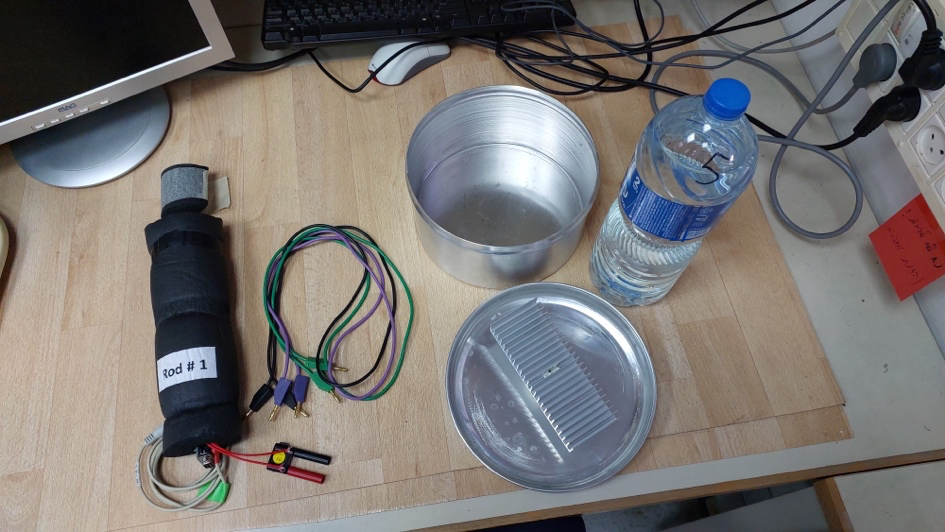
\includegraphics[width=\textwidth]{figures/b-fig1-system.png}};
      \begin{scope}[x={(a.south east)}, y={(a.north west)}]
        \eqlabel{0.25}{0.40}{2} \eqlabel{0.27}{0.14}{3} \eqlabel{0.40}{0.62}{10} \eqlabel{0.53}{0.88}{8}
        \eqlabel{0.62}{0.25}{8} \eqlabel{0.80}{0.62}{9} \eqlabel{0.12}{0.90}{7}
      \end{scope}
    \end{tikzpicture}\\[2pt]
    \begin{tikzpicture}
      \node[inner sep=0, anchor=south west] (c) {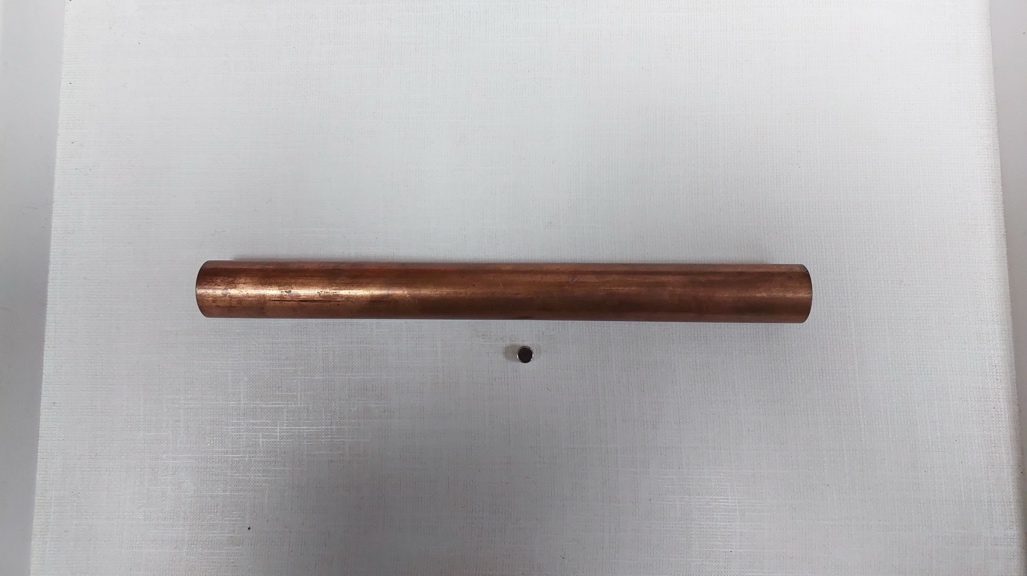
\includegraphics[width=\textwidth]{figures/b-fig3-tube-magnet.jpeg}};
      \begin{scope}[x={(c.south east)}, y={(c.north west)}]
        \eqlabel{0.84}{0.52}{1} \eqlabel{0.50}{0.30}{4}
      \end{scope}
    \end{tikzpicture}
  \end{minipage}\hspace{0.02\textwidth}
  \begin{minipage}[c]{0.31\textwidth}
    \begin{tikzpicture}
      \node[inner sep=0, anchor=south west] (b) {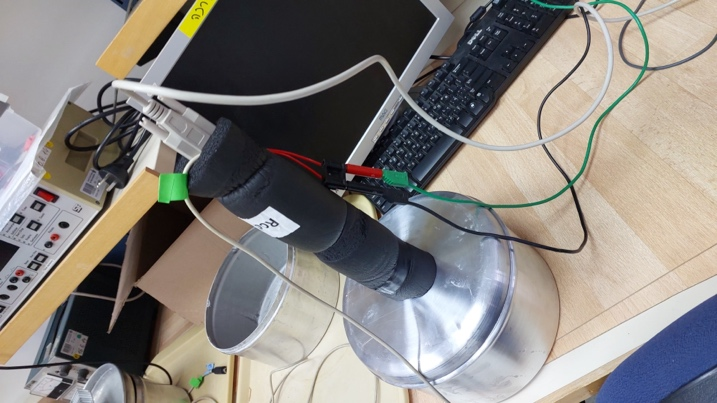
\includegraphics[width=\textwidth, angle=-90]{figures/b-fig2-partb.jpeg}};
      \begin{scope}[x={(b.south east)}, y={(b.north west)}]
        \eqlabel{0.40}{0.55}{2} \eqlabel{0.70}{0.64}{3} \eqlabel{0.45}{0.12}{8} \eqlabel{0.75}{0.80}{10} \eqlabel{0.12}{0.88}{6}
      \end{scope}
    \end{tikzpicture}
  \end{minipage}\hspace{0.02\textwidth}
  % The user's own photo (2026-11-05), cropped from the full bench shot.
  \begin{minipage}[c]{0.17\textwidth}
    \begin{tikzpicture}
      \node[inner sep=0, anchor=south west] (d) {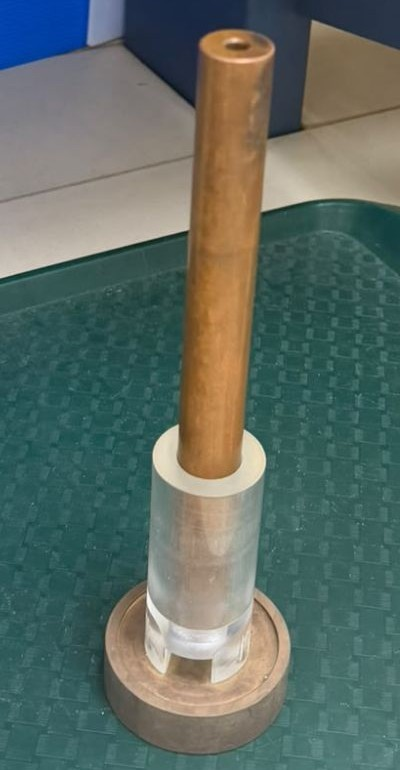
\includegraphics[width=\textwidth]{figures/tube-in-stand.jpeg}};
      \begin{scope}[x={(d.south east)}, y={(d.north west)}]
        \eqlabel{0.80}{0.70}{1} \eqlabel{0.85}{0.30}{16}
      \end{scope}
    \end{tikzpicture}
  \end{minipage}
  \end{otherlanguage}
  \caption{מערכת הניסוי. משמאל למעלה: חלקי המערכת. משמאל למטה: צינור הנחושת של חלק א׳ והמגנט. במרכז: המוט של חלקים ב׳ ו-ג׳ מוברג למכסה הסיר, כפי שהורכב בחלק ב׳. שלוש תמונות אלו מתדריך הניסוי. מימין: הצינור של חלק א׳ מוצב אנכית במתקן הייעודי. המספור תואם לרשימת הציוד.}
  \label{fig:photos}
\end{figure}

% Rod drawing after the briefing's fig. 4: sensor positions in mm. Heater at x = 0: sensor 1 is the
% hottest in the part-b data (36.10 C vs 29.50 C for sensor 8). Water at the far end (part b only).
\begin{figure}[H]
  \centering
  \begin{otherlanguage}{english}
  \begin{tikzpicture}[x=0.065cm, y=0.065cm]
    \fill[gray!35] (0,0) rectangle (200,12);
    \draw (0,0) rectangle (200,12);
    \fill[red!70] (-6,2) rectangle (0,10);
    \node[left, font=\scriptsize] at (-6,6) {\foreignlanguage{hebrew}{נגד חימום} (3)};
    \fill[blue!20] (200,-6) rectangle (226,18); \draw (200,-6) rectangle (226,18);
    \node[font=\scriptsize, align=center] at (213,6) {\foreignlanguage{hebrew}{מים}\\(8, 9)};
    \foreach \p [count=\i] in {15,40,65,90,115,140,165,190} {
      \draw[thick] (\p,12) -- (\p,16);
      \node[above, font=\scriptsize] at (\p,16) {$T_\i$};
      \node[below, font=\tiny] at (\p,0) {\p};
    }
    \draw[->] (0,-9) -- (205,-9) node[right, font=\scriptsize] {$x\ [\mathrm{mm}]$};
    \node[below, font=\tiny] at (0,-9) {0};
  \end{tikzpicture}
  \end{otherlanguage}
  \caption{תרשים סכמטי של מוט הנחושת בחלק ב׳. מיקומי חיישני הטמפרטורה $T_1$ עד $T_8$ במילימטרים, נמדדים מקצה המוט שבו נגד החימום. בקצה השני המוט מוברג למכסה הסיר שבו המים. בחלק ג׳ קצה זה מכוסה בכיסוי המבודד.}
  \label{fig:rod}
\end{figure}

\subsection*{שלבי הניסוי}
\subsubsection*{חלק א׳ -- מוליכות חשמלית}
\begin{enumerate}
  \item מסת המגנט נמדדה במשקל האלקטרוני. המשקל אופס כשעליו כוס הפוכה, והמגנט הונח על הכוס, כדי להרחיק אותו מהמשקל ולמנוע את השפעת השדה המגנטי שלו על המדידה. המסה נמדדה 4 פעמים.
  \item גובה המגנט נמדד בקליבר 4 פעמים. קוטרו לא נמדד בנפרד, כי הוא שווה לגובה.
  \item קוטר התעלה נמדד בקליבר על החוטר 4 פעמים, תחת ההנחה שקוטר החוטר שווה לקוטר התעלה.
  \item הקוטר החיצוני של הצינור נמדד בקליבר 4 פעמים. מכיוון שזווית הקליבר משפיעה על המדידה, זרועות הקליבר הוצמדו למתקן הייעודי העוטף את הצינור, תחת ההנחה ששפתו ניצבת לצינור.
  \item אורך הצינור נמדד בסרגל פעם אחת.
  \item הצינור הוצב אנכית במתקן הייעודי, והמגנט הופל מהקצה העליון של התעלה. זמן הנפילה לאורך הצינור נמדד בשעון העצר 10 פעמים.
\end{enumerate}
זמן הנפילה נמדד 10 פעמים כדי לחשב את זמן הנפילה הממוצע ולהקטין את השגיאה הסטטיסטית, כפי שנקבע בתדריך הניסוי. מספרי החזרות של שאר המדידות נקבעו על ידי מדריך הניסוי.

\subsubsection*{חלק ב׳ -- מוליכות חום}
\begin{enumerate}
  \item המוט הוברג למכסה הסיר, שבו מחליף חום, והסיר מולא במים.
  \item נגד החימום חובר בכבלים לספק הכוח. ספק הכוח הוגבל למתח של $9\U{V}$ ולזרם של $0.7\U{A}$, והופעל באישור המדריך.
  \item המתח והזרם שסופקו לנגד נקראו מצג ספק הכוח.
  \item הקלטת הטמפרטורות של שמונת החיישנים הופעלה בתוכנת המחשב בסמוך להפעלת ספק הכוח, כשהמוט כולו בטמפרטורת החדר. ההקלטה נמשכה $2706\U{s}$, בהתאם להנחיית מדריך הניסוי להקליט לפחות 45 דקות, ובמהלכה תועדה הטמפרטורה של כל החיישנים כל $5\U{s}$. משך זה נדרש כדי שהמוט יגיע למצב קרוב לשיווי משקל תרמי, שבו הטמפרטורה בכל חיישן כמעט אינה משתנה בזמן.
\end{enumerate}

\subsubsection*{חלק ג׳ -- תיקון מסדר ראשון}
\begin{enumerate}
  \item המוט נותק ממכסה הסיר, וקצהו שהיה מוברג לסיר כוסה בכיסוי המבודד. המוט נשאר מחובר לספק הכוח.
  \item קירור: ספק הכוח כובה והקלטת הטמפרטורות הופעלה. המוט התקרר במשך 15 דקות, בהתאם להנחיית מדריך הניסוי.
  \item חימום: בתום 15 הדקות ספק הכוח הופעל, באותן הגדרות כבחלק ב׳, וההקלטה נמשכה 15 דקות נוספות, בהתאם להנחיית מדריך הניסוי.
  \item ההקלטה נמשכה $1834\U{s}$ בסך הכול, ובמהלכה תועדה הטמפרטורה של כל החיישנים כל $5\U{s}$. משכים אלו נדרשו כדי שהתיקון מסדר ראשון בנוסחה~\eqref{eq:pavg} יהיה קירוב טוב דיו.
\end{enumerate}

\section*{תכנון עיבוד התוצאות}
% Split by part like the procedure (user, 2026-11-05).
\subsection*{חלק א׳ -- מוליכות חשמלית}
בחלק זה תחושב המוליכות החשמלית של הנחושת $\sigma$ לפי נוסחה~\eqref{eq:sigma}. לשם כך נדרשים הגדלים הבאים:
\begin{itemize}\setlength{\itemsep}{0pt}\setlength{\parskip}{0pt}
  \item $m$, מסת המגנט: ממוצע ארבע מדידות המשקל.
  \item $t$, זמן הנפילה: ממוצע עשר המדידות בשעון העצר.
  \item $a$, הרדיוס הפנימי של הצינור: מחצית קוטר התעלה, $a = D_{ch}/2$, כאשר $D_{ch}$ הוא ממוצע ארבע המדידות על החוטר.
  \item $w$, עובי דופן הצינור: $w = (D - D_{ch})/2$, כאשר $D$ הוא ממוצע ארבע מדידות הקוטר החיצוני.
  \item $r_m$, רדיוס המגנט: מחצית גובה המגנט $d$ (ממוצע ארבע המדידות), כי קוטר המגנט שווה לגובהו.
  \item $L_0$, אורך הצינור: מדידה אחת בסרגל.
  \item $\mu_0 M = 0.65\U{T}$ ו-$f(d/a) \simeq f(2) \simeq 1.75$: מהרקע התיאורטי.
  \item $g$, תאוצת הכובד: $g = 981\U{cm/s^2}$, מהספרות, ללא שגיאה, כפי שנקבע על ידי מדריך הניסוי.
\end{itemize}
השגיאות בגדלים $m, t, a, r_m, D, D_{ch}$ מתקבלות משקלול של שני מקורות שגיאה, לפי נוסחה (35) בחוברת עיבוד הנתונים: שגיאת הרזולוציה של מכשיר המדידה, תחת הנחת התפלגות אחידה (נוסחה (28) בחוברת), והשגיאה הסטטיסטית (נוסחאות (32) ו-(34) בחוברת).
אורך הצינור $L_0$ נמדד פעם אחת, ולכן שגיאתו היא שגיאת רזולוציה בלבד, לפי נוסחה (28) בחוברת, תחת הנחת התפלגות אחידה בין שנתות הסרגל.
עובי הדופן $w$ מחושב משתי קבוצות מדידה נפרדות, ולכן שגיאתו היא שגיאה עקיפה, המחושבת לפי נוסחה (43) בחוברת:
\begin{equation}\label{eq:dw}
\Delta w = \frac{1}{2}\sqrt{(\Delta D)^2 + (\Delta D_{ch})^2}
\end{equation}
כאשר $\Delta D$ ו-$\Delta D_{ch}$ הן השגיאות בקוטר החיצוני ובקוטר התעלה. עובי הדופן ושגיאתו מוצגים בטבלה~\ref{tab:a-values} בנספח א׳, לצד שאר הגדלים של חלק א׳.
המוליכות החשמלית $\sigma$ מחושבת לפי נוסחה~\eqref{eq:sigma}, ולכן שגיאתה היא שגיאה עקיפה, המחושבת לפי נוסחה (43) בחוברת. הגדלים $g$, $\mu_0 M$ ו-$f(2)$ נתונים ללא שגיאה, ולכן נחשבים מדויקים. הגדלים $a$ ו-$w$ תלויים שניהם ב-$D_{ch}$, ולכן גם השגיאות $\Delta a = \Delta D_{ch}/2$ ו-$\Delta w$ מנוסחה~\eqref{eq:dw} תלויות זו בזו, בעוד שנוסחה (43) מניחה שגיאות בלתי תלויות. לכן $\sigma$ נכתבת כפונקציה של הגדלים שנמדדו ישירות, $D_{ch}$ ו-$D$, על ידי הצבת $a = D_{ch}/2$ ו-$w = (D - D_{ch})/2$, והשגיאה נגזרת לפיהם:
% Tamir (2026-11-15): the second way, sigma in terms of D_ch and D. Numerically checked in analysis.py.
\begin{equation}\label{eq:dsigma}
\Delta\sigma = \sigma\sqrt{\left(\frac{\Delta m}{m}\right)^2 + \left(\frac{\Delta t}{t}\right)^2 + \left(\frac{4\Delta r_m}{r_m}\right)^2 + \left(\frac{\Delta L_0}{L_0}\right)^2 + \left[\left(\frac{2}{D_{ch}} + \frac{1}{D - D_{ch}}\right)\Delta D_{ch}\right]^2 + \left(\frac{\Delta D}{D - D_{ch}}\right)^2}
\end{equation}
כאשר כל הגדלים ושגיאותיהם הוגדרו קודם לכן. השגיאה היחסית ב-$\sigma$ תחושב לפי נוסחה (25) בחוברת, ותיחשב קטנה אם היא קטנה מ-5\%, הסף המקובל בקורס לפי חוברת עיבוד הנתונים. כדי לזהות את מקור השגיאה העיקרי, תחושב גם תרומתו של כל איבר בנוסחה~\eqref{eq:dsigma} לשגיאה היחסית.

\subsection*{חלק ב׳ -- מוליכות חום}
% Slope method (user, 2026-11-09), replacing the single-sensor method of 2026-11-05: kappa from a_1 of fit over all 8 sensors.
ההנחה היא שלאחר 45 דקות של חימום המערכת הגיעה לשיווי משקל תרמי, ולכן ניתן להשתמש בנוסחה~\eqref{eq:linear}, שפותחה תחת הנחה זו.
בחלק זה תחושב מוליכות החום של הנחושת $\kappa$ לפי אותה נוסחה. בנוסחה זו $T(0)$ היא הטמפרטורה בנגד החימום, $P$ הוא ההספק המוזן למוט, $A$ הוא שטח החתך של מוט הנחושת ו-$x$ הוא המרחק מנגד החימום.
בשיווי משקל ההספק קבוע לאורך המוט, ולכן לפי נוסחה~\eqref{eq:linear} הטמפרטורה תלויה לינארית במיקום. לכן תבוצע התאמה לינארית של הטמפרטורות שמודדים שמונת החיישנים כפונקציה של מיקומם:
\begin{equation}\label{eq:fitb}
T = a_1 x + a_0
\end{equation}
כאשר $x$ הוא מיקום החיישן ו-$T$ היא הטמפרטורה שהוא מודד. מיקומי החיישנים קבועים במבנה המוט (איור~\ref{fig:rod}) ולא נמדדו בניסוי, ולכן אין בהם חזרות, ושגיאתם היא $2\U{mm}$, כפי שנקבע על ידי מדריך הניסוי. כל נקודה בהתאמה היא קריאה אחת של חיישן, ושגיאתה $0.002\U{K}$, כפי שנקבע על ידי מדריך הניסוי. מדדי ההתאמה יבחנו אם הערכת שגיאות זו סבירה. לפי נוסחה~\eqref{eq:linear}, נקודת החיתוך היא $a_0 = T(0)$, והשיפוע הוא $a_1 = -\frac{P}{\kappa A}$. ההתאמה תתבצע על הטמפרטורות שנמדדו במדידה האחרונה, לאחר 45 דקות של חימום, שבה המערכת קרובה ביותר לשיווי משקל. כדי לבדוק שהמערכת אכן בשיווי משקל, ההתאמה תחזור גם בשתי מדידות מוקדמות יותר, 100 ו-200 שניות לפני המדידה האחרונה, כפי שנקבע בתדריך הניסוי. בשיווי משקל השיפועים בשלוש ההתאמות צפויים להיות שווים, וההשוואה ביניהם תיעשה באמצעות מדד $N_\sigma$ (נוסחה (51) בחוברת).
מהעברת אגפים בביטוי לשיפוע נקבל:
\begin{equation}\label{eq:kappa}
\kappa = -\frac{P}{A a_1}
\end{equation}

לחישוב $\kappa$ לפי נוסחה~\eqref{eq:kappa} נדרשים הגדלים הבאים:
\begin{itemize}\setlength{\itemsep}{0pt}\setlength{\parskip}{0pt}
  \item $P$, ההספק המוזן למוט: $P = VI$, כאשר $V$ ו-$I$ הם המתח והזרם שנקראו מצג ספק הכוח.
  \item $A$, שטח החתך של המוט: $A = \frac{\pi}{4}D^2$, כאשר $D$ הוא הקוטר החיצוני שנמדד בחלק א׳.
  \item $a_1$: שיפוע התאמה~\eqref{eq:fitb}.
\end{itemize}

המתח $V$ והזרם $I$ נקראו פעם אחת מצג ספק הכוח, ולכן שגיאתם היא שגיאת רזולוציה בלבד, לפי נוסחה (28) בחוברת, תחת הנחת התפלגות אחידה. השגיאה בשיפוע $\Delta a_1$ מתקבלת מההתאמה, והשגיאה ב-$D$ חושבה בחלק א׳. מוליכות החום מחושבת לפי נוסחה~\eqref{eq:kappa}, ולכן שגיאתה היא שגיאה עקיפה לפי נוסחה (43) בחוברת. לאחר הצבת $P$ ו-$A$ מתקבל:
\begin{equation}\label{eq:dkappa}
\Delta\kappa = \kappa\sqrt{\left(\frac{\Delta V}{V}\right)^2 + \left(\frac{\Delta I}{I}\right)^2 + \left(\frac{\Delta a_1}{a_1}\right)^2 + \left(\frac{2\Delta D}{D}\right)^2}
\end{equation}
כאשר כל הגדלים ושגיאותיהם הוגדרו קודם לכן.


מוליכות החום שחושבה והמוליכות החשמלית ישמשו לחישוב קבוע לורנץ, לפי נוסחה~\eqref{eq:wf}:
\begin{equation}\label{eq:lorenz}
L = \frac{\kappa}{\sigma T}
\end{equation}
כאשר $T$ היא הטמפרטורה הממוצעת של המתכת. מאחר שהמדידות נעשו בטמפרטורות שונות, לפי מדריך הניסוי היא מוערכת כטמפרטורת החדר, $24\U{^\circ C} = 297.15\U{K}$, בשגיאה של $1\U{K}$. שגיאתו של $L$ היא שגיאה עקיפה לפי נוסחה (43) בחוברת. $\kappa$ ו-$\sigma$ תלויות שתיהן בקוטר $D$, ולכן אינן בלתי תלויות. לכן, כמו בנוסחה~\eqref{eq:dsigma}, $L$ נכתב כפונקציה של הגדלים שנמדדו ישירות, על ידי הצבת נוסחאות~\eqref{eq:sigma} ו-\eqref{eq:kappa}, $P = VI$ ו-$A = \frac{\pi}{4}D^2$, והשגיאה נגזרת לפיהם:
% Same rule as (7) (Tamir 2026-11-15), user chose it for (12) 2026-11-15. Checked against the simple form: same rounding.
\begin{equation}\label{eq:dlorenz}
\begin{split}
\Delta L = L\Bigg[&\left(\frac{\Delta V}{V}\right)^2 + \left(\frac{\Delta I}{I}\right)^2 + \left(\frac{\Delta a_1}{a_1}\right)^2 + \left(\frac{\Delta m}{m}\right)^2 + \left(\frac{\Delta t}{t}\right)^2 + \left(\frac{4\Delta r_m}{r_m}\right)^2 + \left(\frac{\Delta L_0}{L_0}\right)^2 + \left(\frac{\Delta T}{T}\right)^2 \\
&+ \left[\left(\frac{1}{D - D_{ch}} - \frac{2}{D}\right)\Delta D\right]^2 + \left[\left(\frac{2}{D_{ch}} + \frac{1}{D - D_{ch}}\right)\Delta D_{ch}\right]^2\Bigg]^{1/2}
\end{split}
\end{equation}
הערך שיתקבל יושווה לערך התיאורטי $L = 2.44 \cdot 10^{-8}\U{V^2/K^2}$ מהרקע התיאורטי, באמצעות מדד $N_\sigma$ לפי נוסחה (52) בחוברת, כי לערך התיאורטי אין שגיאה. הערכים יתאימו אם $N_\sigma \le 3$.

\subsection*{חלק ג׳ -- תיקון מסדר ראשון}
% Choices (user, 2026-11-14), each explained in the text: sensor 4; cooling = whole interval; heating = 3-6 min
% after switch-on (transient ends at 3 min: sensor rates within 4% from then on); T_exp = last 200 s of part b.
בחלק זה תתוקן מוליכות החום שחושבה בחלק ב׳: במקום ההספק המוזן למוט $P_{in} = VI$ ישמש ההספק הממוצע לאורך המוט $P_{avg}$ לפי נוסחה~\eqref{eq:pavg}, שמביא בחשבון את ההספק שאבד לסביבה ואת ההספק שנבלע במוט. שלושת קצבי שינוי הטמפרטורה בנוסחה זו יחושבו מחיישן אחד מאמצע המוט, לפי הנחיית מדריך הניסוי. מיקומו של חיישן 4, $90\U{mm}$, הוא הקרוב ביותר לאמצע המוט, ולכן הקצבים יחושבו ממנו.

כל קצב יתקבל מהתאמה לינארית של טמפרטורת החיישן כפונקציה של הזמן:
\begin{equation}\label{eq:fitc}
T = b_1 t + b_0
\end{equation}
כאשר $t$ הוא הזמן, $T$ היא הטמפרטורה שמדד החיישן, והקצב הוא השיפוע $b_1$. שגיאת הטמפרטורה היא $0.002\U{K}$, כמו בחלק ב׳. תוכנת ההקלטה מתעדת את הזמן ברזולוציה של $0.001\U{s}$, ולכן שגיאת הזמן היא שגיאת רזולוציה. היא מחושבת לפי נוסחה (28) בחוברת, תחת הנחת התפלגות אחידה. ההתאמות ייעשו במקטעים הבאים:
\begin{itemize}\setlength{\itemsep}{0pt}\setlength{\parskip}{0pt}
  \item $\dot{T}_{cool}$: כל מקטע הקירור, 15 הדקות שבהן ספק הכוח היה כבוי, כדי להשתמש בכל המדידות שבו.
  \item $\dot{T}_{heat}$: מהדקה השלישית עד הדקה ה-12 לאחר הפעלת ספק הכוח. לפי הנחיית מדריך הניסוי, המקטע רחוק מרגע הפעלת ספק הכוח ונמצא באמצע זמן החימום, באזור שבו השינוי בטמפרטורה נראה לינארי, ויש בו מספיק נקודות. בשלוש הדקות הראשונות לאחר הפעלת ספק הכוח קצבי החימום של החיישנים שונים זה מזה, ומהדקה השלישית כל החיישנים מתחממים בקירוב באותו קצב. לכן המקטע מתחיל בדקה השלישית, ומרכזו באמצע זמן החימום, בדקה ה-7.5.
  \item $\dot{T}_{exp}$: 200 השניות האחרונות של ההקלטה בחלק ב׳. $\dot{T}_{exp}$ הוא קצב שינוי הטמפרטורה בזמן המדידות שמהן חושבה מוליכות החום. שלוש ההתאמות של חלק ב׳ נעשו בתחילת מקטע זה, באמצעו ובסופו, ולכן הקצב יחושב בו.
\end{itemize}

שגיאת כל קצב היא שגיאת השיפוע מההתאמה. ההספק הממוצע מחושב לפי נוסחה~\eqref{eq:pavg}, ולכן שגיאתו היא שגיאה עקיפה לפי נוסחה (43) בחוברת. לאחר הצבת $P_{in} = VI$ מתקבל:
\begin{equation}\label{eq:dpavg}
\begin{split}
\Delta P_{avg} = \Bigg[ & P_{avg}^2\left(\left(\frac{\Delta V}{V}\right)^2 + \left(\frac{\Delta I}{I}\right)^2\right) \\
& + \left(\frac{P_{in}}{2(\dot{T}_{heat} - \dot{T}_{cool})}\right)^2 \left( (\Delta\dot{T}_{exp})^2 + \left(\frac{\dot{T}_{heat} - \dot{T}_{exp}}{\dot{T}_{heat} - \dot{T}_{cool}}\,\Delta\dot{T}_{cool}\right)^2 + \left(\frac{\dot{T}_{exp} - \dot{T}_{cool}}{\dot{T}_{heat} - \dot{T}_{cool}}\,\Delta\dot{T}_{heat}\right)^2 \right) \Bigg]^{\frac{1}{2}}
\end{split}
\end{equation}
כאשר כל הגדלים ושגיאותיהם הוגדרו קודם לכן.

מוליכות החום המתוקנת, $\kappa_c$, תחושב לפי נוסחה~\eqref{eq:kappa}, כאשר $P_{avg}$ מחליף את $P$. השגיאה ב-$P_{avg}$ לפי נוסחה~\eqref{eq:dpavg} כבר כוללת את השגיאות ב-$V$ וב-$I$, דרך $P_{in} = VI$. לכן בנוסחה~\eqref{eq:dkappa} האיבר $\left(\frac{\Delta P_{avg}}{P_{avg}}\right)^2$ מחליף את שני האיברים של $V$ ושל $I$, ושגיאת מוליכות החום המתוקנת היא:
\begin{equation}\label{eq:dkappac}
\Delta\kappa_c = \kappa_c\sqrt{\left(\frac{\Delta P_{avg}}{P_{avg}}\right)^2 + \left(\frac{\Delta a_1}{a_1}\right)^2 + \left(\frac{2\Delta D}{D}\right)^2}
\end{equation}
לבסוף, קבוע לורנץ $L_c$ יחושב שוב לפי נוסחה~\eqref{eq:lorenz} עם $\kappa_c$, ושגיאתו מתקבלת מנוסחה~\eqref{eq:dlorenz} באותה החלפה:
\begin{equation}\label{eq:dlorenzc}
\begin{split}
\Delta L_c = L_c\Bigg[&\left(\frac{\Delta P_{avg}}{P_{avg}}\right)^2 + \left(\frac{\Delta a_1}{a_1}\right)^2 + \left(\frac{\Delta m}{m}\right)^2 + \left(\frac{\Delta t}{t}\right)^2 + \left(\frac{4\Delta r_m}{r_m}\right)^2 + \left(\frac{\Delta L_0}{L_0}\right)^2 + \left(\frac{\Delta T}{T}\right)^2 \\
&+ \left[\left(\frac{1}{D - D_{ch}} - \frac{2}{D}\right)\Delta D\right]^2 + \left[\left(\frac{2}{D_{ch}} + \frac{1}{D - D_{ch}}\right)\Delta D_{ch}\right]^2\Bigg]^{1/2}
\end{split}
\end{equation}
כאשר כל הגדלים ושגיאותיהם הוגדרו קודם לכן. גם $L_c$ יושווה לערך התיאורטי כמו בחלק ב׳.

\section*{תוצאות}
\subsection*{חלק א׳ -- מוליכות חשמלית}
% (7) in the D_ch/D form per Tamir (2026-11-15).
המוליכות החשמלית של הנחושת שחושבה לפי נוסחה~\eqref{eq:sigma} היא $\sigma = \SigmaVal\U{S/m}$ (ביחידות \textenglish{SI} בסיסיות, $\mathrm{S/m} = \mathrm{kg^{-1}\cdot m^{-3}\cdot s^{3}\cdot A^{2}}$), בשגיאה יחסית של $\SigmaRel$, קטנה מהסף העליון המקובל של 5\% לפי חוברת עיבוד הנתונים. מבין האיברים בנוסחה~\eqref{eq:dsigma}, האיבר שמייצג את השגיאה ברדיוס המגנט, $\frac{4\Delta r_m}{r_m}$, הוא הגדול ביותר, $\ATermR$, ואחריו האיבר שמייצג את השגיאה בקוטר התעלה, $\left(\frac{2}{D_{ch}} + \frac{1}{D - D_{ch}}\right)\Delta D_{ch}$, $\ATermDch$. כל אחד משאר האיברים אינו עולה על $\ATermRestMax$. ארבע מדידות המסה נתנו אותו ערך, ולכן שגיאת המסה היא שגיאת רזולוציה בלבד. עשר מדידות זמן הנפילה נעו בין $\ATMin\U{s}$ ל-$\ATMax\U{s}$. הגדלים ששימשו לחישוב ושגיאותיהם מרוכזים בטבלה~\ref{tab:a-values} בנספח א׳.

\subsection*{חלק ב׳ -- מוליכות חום}
\begin{figure}[H]
  \centering
  % RTL: the first minipage lands on the right, so the fit (read first) comes first.
  \begin{minipage}[t]{0.48\textwidth}
    \centering
    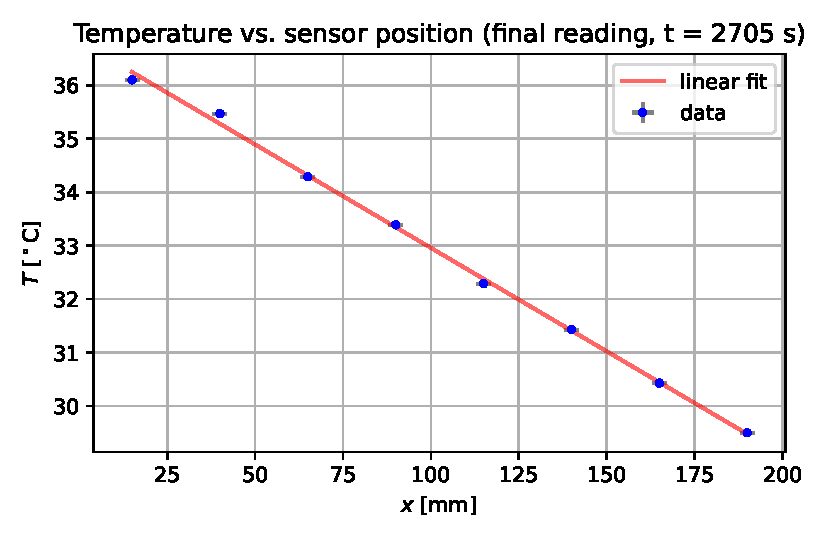
\includegraphics[width=\textwidth]{figures/b_fit.pdf}
    \caption{הטמפרטורה $T$ במעלות צלזיוס כתלות במיקום החיישן $x$ במילימטרים, במדידה האחרונה ($t = \BLastTime\U{s}$), וההתאמה הלינארית לפי נוסחה~\eqref{eq:fitb}. צלבי השגיאה מציגים את $\Delta x$ ואת $\Delta T$ (צלב השגיאה האנכי קטן מכדי להיראות).}
    \label{fig:b-fit}
  \end{minipage}\hfill
  \begin{minipage}[t]{0.48\textwidth}
    \centering
    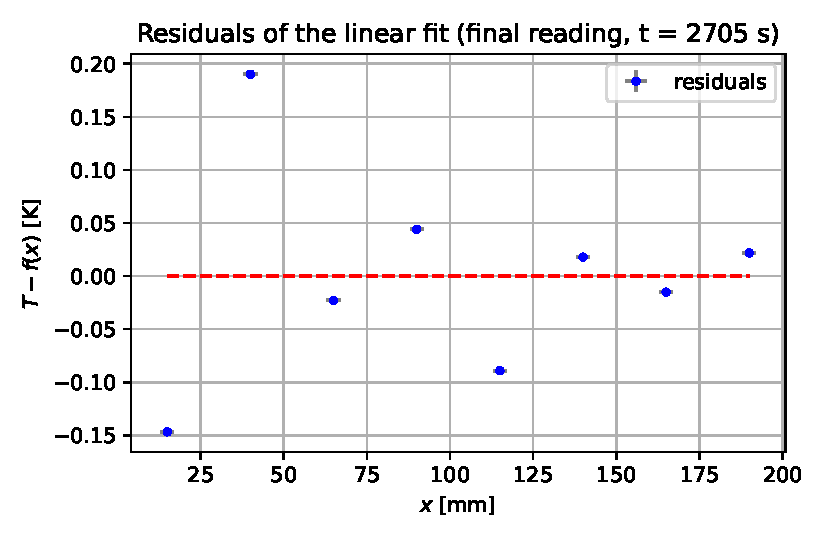
\includegraphics[width=\textwidth]{figures/b_res.pdf}
    \caption{גרף השארים של ההתאמה: ההפרש בין הטמפרטורה הנמדדת לבין ערך פונקציית ההתאמה, בקלווין, כתלות ב-$x$ במילימטרים. צלבי השגיאה מציגים את $\Delta T$ ו-$\Delta x$ בלבד (צלב השגיאה האנכי קטן מכדי להיראות). השגיאה האפקטיבית של כל נקודה, הכוללת את תרומת שגיאת המיקום דרך השיפוע, $|a_1|\Delta x = \BXErrK\U{K}$, אינה מוצגת בגרף.}
    \label{fig:b-res}
  \end{minipage}
\end{figure}
גרף ההתאמה במדידה האחרונה וגרף השארים שלה מוצגים באיור~\ref{fig:b-fit} ובאיור~\ref{fig:b-res}.\footnote{הטמפרטורות בגרפי ההתאמה מוצגות במעלות צלזיוס, כי כך נרשמו בתוכנת ההקלטה. השארים הם הפרשי טמפרטורה, ולכן הם מוצגים בקלווין, בגרף זה ובגרפי השארים שבהמשך; הפרש של $1\U{K}$ שווה להפרש של $1\U{^\circ C}$.} ההתאמה חזרה גם בשתי מדידות מוקדמות יותר, 100 ו-200 שניות לפני המדידה האחרונה, לבדיקת שיווי המשקל. גרפי ההתאמה והשארים של שתי ההתאמות המוקדמות מוצגים בנספח ב׳. דפוס השארים חוזר בשלוש ההתאמות: בכל חיישן סימן השארית זהה בשלושתן, ובכולן השארים הגדולים ביותר הם של חיישנים 1 ו-2 (איורים~\ref{fig:b-res}, \ref{fig:b-res-mid} ו-\ref{fig:b-res-early}). הפרמטרים של שלוש ההתאמות, מדדי טיב ההתאמה שלהן ($\chi^2_{red}$ ו-\textenglish{p-value}) ומוליכות החום שחולצה מהן מרוכזים בטבלה~\ref{tab:b-results}.

בגרף ההתאמה, הטמפרטורה יורדת עם המרחק מנגד החימום, ונקודות המדידה נמצאות על קו ההתאמה או בסמוך אליו. השיפוע $a_1$ שלילי, כצפוי לפי נוסחה~\eqref{eq:linear}.

בגרף השארים, סימני השארים מתחלפים לאורך המוט, ולא ניכרת בהם מגמה. השארים הגדולים ביותר הם של שני החיישנים הקרובים לנגד החימום. צלבי השגיאה בגרף קטנים בהרבה מהשארים, כי $\Delta T = \TErr\U{K}$, ואילו שגיאת המיקום, דרך השיפוע, תורמת כ-$\BXErrK\U{K}$ לשגיאה האפקטיבית של כל נקודה בהתאמה. ביחידות של שגיאה אפקטיבית זו, כל השארים רחוקים מקו האפס פחות משלוש שגיאות.

בקריאה הראשונה של חלק ב׳, כשכל החיישנים עדיין בטמפרטורת החדר, קריאות החיישנים שונות מהממוצע שלהן בעד $\DOffsetMax\U{K}$, באותו דפוס סימנים של השארים. הפרשים אלו עשויים להיות שגיאה שיטתית של כל חיישן. כדי לבדוק אם הם מסבירים את השארים, הוחסרה ההסטה של כל חיישן מהשארית שלו בהתאמה במדידה האחרונה. החסרה זו דומה לתיקון שגיאה שיטתית המתואר בפרק השגיאה השיטתית בחוברת עיבוד הנתונים. לאחר החסרת ההסטות מהשאריות, השארית בחיישנים 3 עד 8 היא עד $\DCorrRestMax\U{K}$, ובחיישנים 1 ו-2 נשארות שאריות של $-\DCorrOne\U{K}$ ו-$+\DCorrTwo\U{K}$, בהתאמה.

עם זאת, ההסטות נמדדו בטמפרטורת החדר בלבד, בעוד שהקריאות בהתאמה נמדדו בטמפרטורות גבוהות יותר, ולא ניתן היה לבדוק אם ההסטה של כל חיישן נשארת קבועה כשהטמפרטורה משתנה. בנוסף, כל הסטה נקבעה מקריאה אחת בלבד. לכן לא ניתן לתקן את הקריאות עצמן באמצעות ההסטות, וההתאמה והערכים המדווחים חושבו מהקריאות המקוריות, ללא תיקון.

\begin{table}[H]
  \centering
  \renewcommand{\arraystretch}{1.3}
  \begin{tabular}{|c|c|c|c|}
    \hline
     & $t = \BLastTime\U{s}$ & $t = \BMidTime\U{s}$ & $t = \BEarlyTime\U{s}$ \\
    \hline
    $a_0\ [^\circ\mathrm{C}]$ & $\BLastAZero$ & $\BMidAZero$ & $\BEarlyAZero$ \\
    \hline
    $a_1\ [\mathrm{K/m}]$ & $\BLastAOne$ & $\BMidAOne$ & $\BEarlyAOne$ \\
    \hline
    $\frac{\Delta a_1}{a_1}$ & $\BLastAOneRel$ & $\BMidAOneRel$ & $\BEarlyAOneRel$ \\
    \hline
    $\chi^2_{red}$ & $\BLastChi$ & $\BMidChi$ & $\BEarlyChi$ \\
    \hline
    \textenglish{p-value} & $\BLastP$ & $\BMidP$ & $\BEarlyP$ \\
    \hline
    $\kappa\ [\mathrm{W/(m\cdot K)}]$ & $\BLastKappa$ & $\BMidKappa$ & $\BEarlyKappa$ \\
    \hline
    $\frac{\Delta\kappa}{\kappa}$ & $\BLastKappaRel$ & $\BMidKappaRel$ & $\BEarlyKappaRel$ \\
    \hline
  \end{tabular}
  \caption{הפרמטרים של ההתאמה לפי נוסחה~\eqref{eq:fitb}, מדדי טיב ההתאמה ומוליכות החום לפי נוסחאות~\eqref{eq:kappa} ו-\eqref{eq:dkappa}, במדידה האחרונה ובשתי מדידות מוקדמות יותר.}
  \label{tab:b-results}
\end{table}
בשלוש ההתאמות $\chi^2_{red}$ קרוב ל-2, וה-\textenglish{p-value} בין 0.05 ל-0.95. ערך \textenglish{p-value} זה מעיד שערך $\chi^2_{red}$ שהתקבל סביר עבור שש דרגות החופש של ההתאמה, אף שהוא גדול מ-1. בשלוש ההתאמות ה-\textenglish{p-value} קרוב לגבול התחתון של התחום, 0.05. מוליכות החום במדידה האחרונה היא $\kappa = \BLastKappa\U{W/(m\cdot K)}$. מדד $N_\sigma$ בין השיפועים הוא $\BNsigmaAB$ בין המדידה האחרונה למדידה שלפניה ב-100 שניות, $\BNsigmaAC$ בין המדידה האחרונה למדידה שלפניה ב-200 שניות, ו-$\BNsigmaBC$ בין שתי המדידות המוקדמות, כולם קטנים מ-3.

קבוע לורנץ שחושב ממוליכות חום זו לפי נוסחאות~\eqref{eq:lorenz} ו-\eqref{eq:dlorenz} הוא $L = \BLorenz\U{V^2/K^2}$, בשגיאה יחסית של $\BLorenzRel$, ומדד $N_\sigma$ ביחס לערך התיאורטי $L = 2.44 \cdot 10^{-8}\U{V^2/K^2}$ הוא $\BLorenzNsigma$, החורג מהסף המקובל של 3. לכן ערך זה אינו תואם לערך התיאורטי.

\subsection*{חלק ג׳ -- תיקון מסדר ראשון}
\begin{figure}[H]
  \centering
  \begin{minipage}[t]{0.48\textwidth}
    \centering
    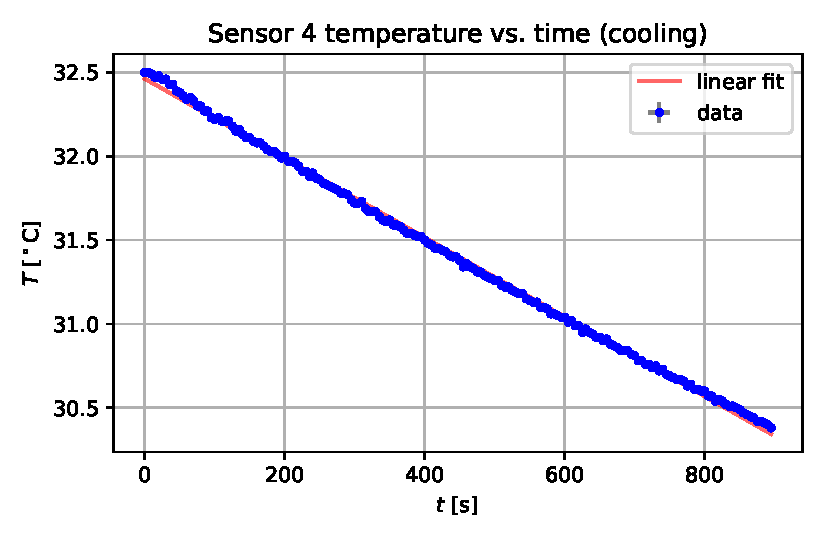
\includegraphics[width=\textwidth]{figures/c_cool_fit.pdf}
    \caption{הטמפרטורה $T$ שמדד חיישן 4 במעלות צלזיוס כתלות בזמן $t$ בשניות, במקטע הקירור, וההתאמה הלינארית לפי נוסחה~\eqref{eq:fitc}.}
    \label{fig:c-cool-fit}
  \end{minipage}\hfill
  \begin{minipage}[t]{0.48\textwidth}
    \centering
    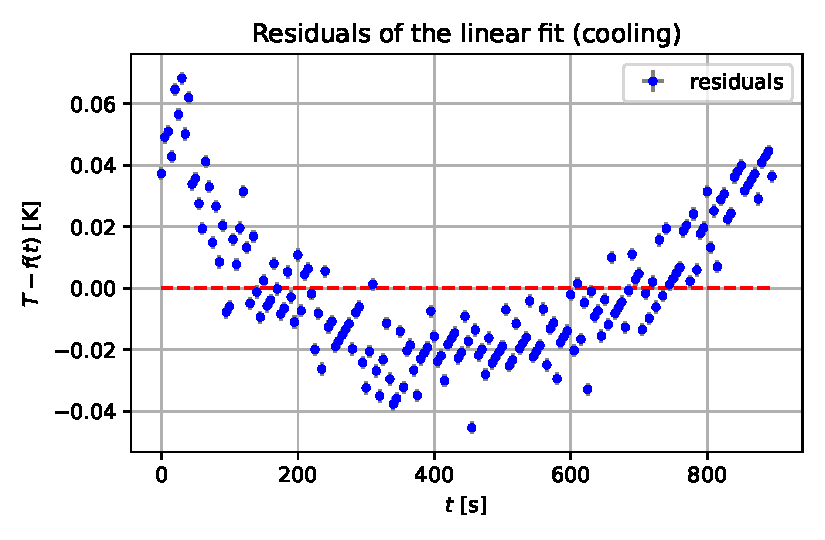
\includegraphics[width=\textwidth]{figures/c_cool_res.pdf}
    \caption{גרף השארים של ההתאמה: ההפרש בין הטמפרטורה הנמדדת לבין ערך פונקציית ההתאמה, בקלווין, כתלות ב-$t$ בשניות. צלבי השגיאה מציגים את $\Delta T$ ו-$\Delta t$ בלבד (שניהם קטנים מכדי להיראות).}
    \label{fig:c-cool-res}
  \end{minipage}
\end{figure}
\begin{figure}[H]
  \centering
  \begin{minipage}[t]{0.48\textwidth}
    \centering
    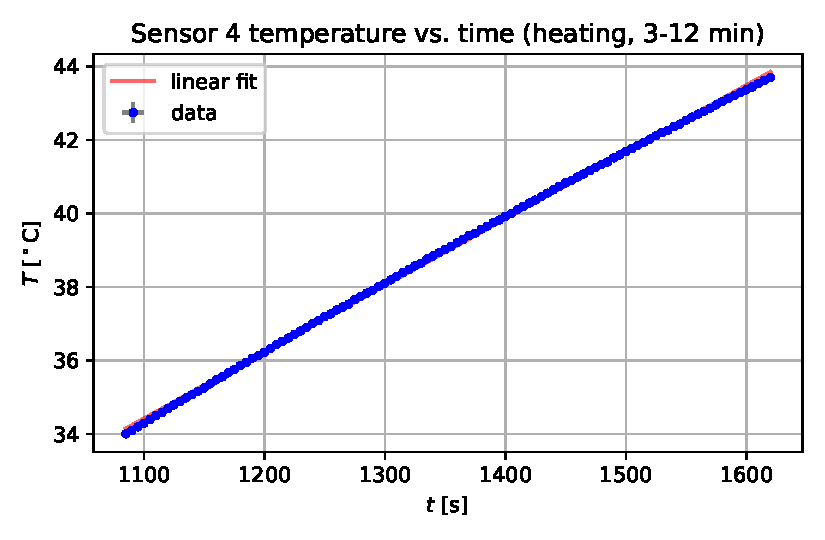
\includegraphics[width=\textwidth]{figures/c_heat_fit.pdf}
    \caption{הטמפרטורה $T$ שמדד חיישן 4 במעלות צלזיוס כתלות בזמן $t$ בשניות, מהדקה השלישית עד הדקה ה-12 לאחר הפעלת ספק הכוח, וההתאמה הלינארית לפי נוסחה~\eqref{eq:fitc}.}
    \label{fig:c-heat-fit}
  \end{minipage}\hfill
  \begin{minipage}[t]{0.48\textwidth}
    \centering
    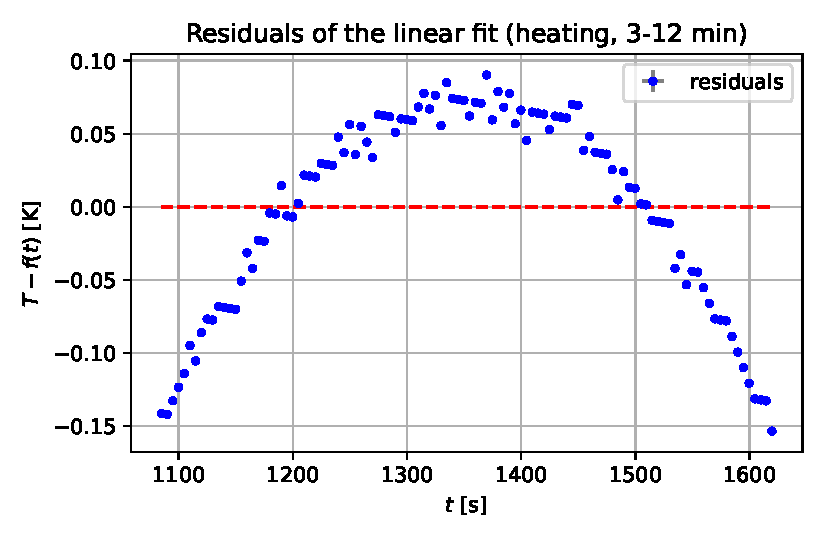
\includegraphics[width=\textwidth]{figures/c_heat_res.pdf}
    \caption{גרף השארים של ההתאמה: ההפרש בין הטמפרטורה הנמדדת לבין ערך פונקציית ההתאמה, בקלווין, כתלות ב-$t$ בשניות. צלבי השגיאה מציגים את $\Delta T$ ו-$\Delta t$ בלבד (שניהם קטנים מכדי להיראות).}
    \label{fig:c-heat-res}
  \end{minipage}
\end{figure}
\begin{figure}[H]
  \centering
  \begin{minipage}[t]{0.48\textwidth}
    \centering
    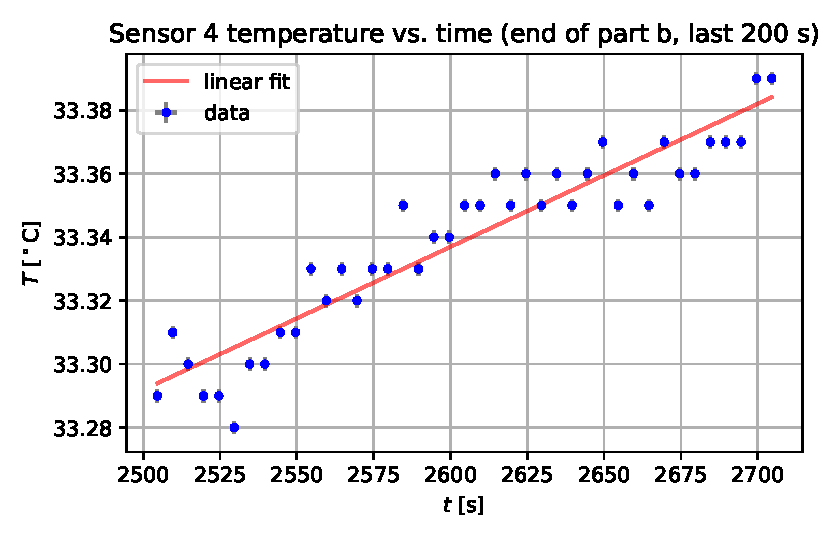
\includegraphics[width=\textwidth]{figures/c_exp_fit.pdf}
    \caption{הטמפרטורה $T$ שמדד חיישן 4 במעלות צלזיוס כתלות בזמן $t$ בשניות, ב-200 השניות האחרונות של ההקלטה בחלק ב׳, וההתאמה הלינארית לפי נוסחה~\eqref{eq:fitc}.}
    \label{fig:c-exp-fit}
  \end{minipage}\hfill
  \begin{minipage}[t]{0.48\textwidth}
    \centering
    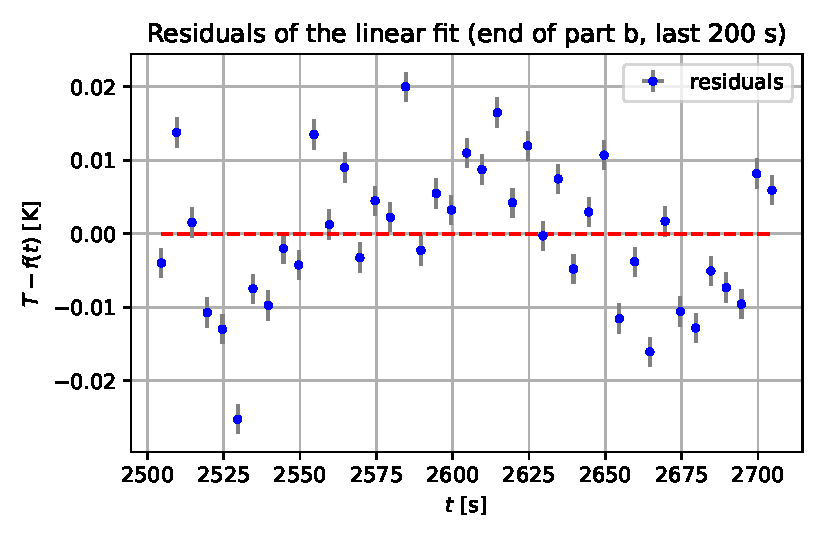
\includegraphics[width=\textwidth]{figures/c_exp_res.pdf}
    \caption{גרף השארים של ההתאמה: ההפרש בין הטמפרטורה הנמדדת לבין ערך פונקציית ההתאמה, בקלווין, כתלות ב-$t$ בשניות. צלבי השגיאה מציגים את $\Delta T$ ו-$\Delta t$ בלבד (צלב השגיאה האופקי קטן מכדי להיראות).}
    \label{fig:c-exp-res}
  \end{minipage}
\end{figure}

גרפי שלוש ההתאמות לחישוב קצבי שינוי הטמפרטורה וגרפי השארים שלהן מוצגים באיורים~\ref{fig:c-cool-fit} עד~\ref{fig:c-exp-res}. הפרמטרים של ההתאמות ומדדי טיב ההתאמה שלהן ($\chi^2_{red}$ ו-\textenglish{p-value}) מרוכזים בטבלה~\ref{tab:c-results}.

בגרפי ההתאמה, במקטע הקירור הטמפרטורה יורדת עם הזמן, ובמקטע החימום ובסוף חלק ב׳ היא עולה. בשלושת הגרפים נקודות המדידה נמצאות על קו ההתאמה או בסמוך אליו.

באיור~\ref{fig:c-cool-res} (שארי הקירור) השארים מסודרים בצורה דמוית פרבולה קמורה מטה, ובאיור~\ref{fig:c-heat-res} (שארי החימום) בצורה דמוית פרבולה קמורה מעלה. גם באיור~\ref{fig:c-exp-res} (שארי סוף חלק ב׳) השארים מסודרים בצורה דמוית פרבולה קמורה מעלה, אך היא פחות מובהקת, כי פיזור השארים סביבה גדול ביחס לגובהה. בשלושת האיורים צלבי השגיאה קטנים בהרבה מהשארים. באיור~\ref{fig:c-cool-res}, $\CCoolFracThree$ מהשארים רחוקים מקו האפס יותר משלוש שגיאות, ובאיור~\ref{fig:c-heat-res}, $\CHeatFracThree$ מהם. באיור~\ref{fig:c-exp-res}, $\CExpFracThree$ מהשארים רחוקים מקו האפס יותר משלוש שגיאות.

האחוזים הגבוהים של שארים הרחוקים מקו האפס יותר משלוש שגיאות, בשלושת גרפי השארים, מעידים שהשגיאות קטנות בהרבה ממרחק הנקודות מקו ההתאמה, כלומר הערכת חסר של השגיאות או מודל שאינו מתאר את המדידות, בהתאם לערכי $\chi^2_{red}$ הגדולים בטבלה~\ref{tab:c-results}. יחד עם הצורה דמוית הפרבולה של השארים, הדבר מראה שההתאמות הלינאריות, עם השגיאות שנקבעו, אינן מתארות היטב את המדידות. הסיבות האפשריות לכך נדונות בדיון.

\begin{table}[H]
  \centering
  \renewcommand{\arraystretch}{1.3}
  \begin{tabular}{|c|c|c|c|}
    \hline
     & קירור & חימום & סוף חלק ב׳ \\
    \hline
    מספר נקודות & $\CCoolN$ & $\CHeatN$ & $\CExpN$ \\
    \hline
    קצב, $b_1\ [10^{-3}\,\mathrm{K/s}]$ & $\CCoolRate$ & $\CHeatRate$ & $\CExpRate$ \\
    \hline
    $\frac{\Delta b_1}{b_1}$ & $\CCoolRateRel$ & $\CHeatRateRel$ & $\CExpRateRel$ \\
    \hline
    $\chi^2_{red}$ & $\CCoolChi$ & $\CHeatChi$ & $\CExpChi$ \\
    \hline
    \textenglish{p-value} & $\CCoolP$ & $\CHeatP$ & $\CExpP$ \\
    \hline
  \end{tabular}
  \caption{קצבי שינוי הטמפרטורה $\dot{T}_{cool}$, $\dot{T}_{heat}$ ו-$\dot{T}_{exp}$, השיפועים $b_1$ של ההתאמות לפי נוסחה~\eqref{eq:fitc}, ומדדי טיב ההתאמה. ערכי \textenglish{p-value} הקטנים מ-$10^{-100}$ מוצגים כחסם עליון בלבד.}
  \label{tab:c-results}
\end{table}
בשלוש ההתאמות $\chi^2_{red}$ גדול בהרבה מ-1, וה-\textenglish{p-value} קרוב לאפס. ערך \textenglish{p-value} זה מעיד שערך $\chi^2_{red}$ שהתקבל גדול מהצפוי עבור מספר דרגות החופש של כל התאמה.

ההספק המוזן למוט הוא $P_{in} = \CPin\U{W}$, וההספק הממוצע לפי נוסחה~\eqref{eq:pavg} הוא $P_{avg} = \CPavg\U{W}$, בשגיאה יחסית של $\CPavgRel$. מוליכות החום המתוקנת היא $\kappa_c = \CKappa\U{W/(m\cdot K)}$, בשגיאה יחסית של $\CKappaRel$.

קבוע לורנץ שחושב ממוליכות החום המתוקנת הוא $L_c = \CLorenz\U{V^2/K^2}$, בשגיאה יחסית של $\CLorenzRel$, ומדד $N_\sigma$ ביחס לערך התיאורטי הוא $\CLorenzNsigma$, החורג מהסף המקובל של 3. לכן ערך זה אינו תואם לערך התיאורטי.

\section*{דיון}
% Bases (user rule 2026-11-14): theory files, instructor, data observations. No outside physics.
% One idea per bullet (user, 2026-11-15).
\subsection*{עמידה במטרות}
\begin{itemize}\setlength{\itemsep}{2pt}\setlength{\parskip}{0pt}
  \item דיוק המדידות: המוליכות החשמלית ומוליכות החום נמדדו בשגיאות יחסיות של $\SigmaRel$ ו-$\BLastKappaRel$, קטנות מהסף העליון המקובל של 5\% לפי חוברת עיבוד הנתונים.
  \item קבוע לורנץ: אף שהשגיאות היחסיות במוליכויות קטנות, קבוע לורנץ שחושב מהן אינו תואם לערך התיאורטי, הן ללא התיקון והן עמו.
  \begin{itemize}\setlength{\itemsep}{0pt}\setlength{\parskip}{0pt}
    \item ללא התיקון, $N_\sigma = \BLorenzNsigma$, החורג מהסף המקובל של 3.
    \item יתרה מזאת, עם התיקון קבוע לורנץ קטן יותר, והפער מהערך התיאורטי גדל: $N_\sigma = \CLorenzNsigma$.
    \item לכן מטרת הניסוי, לבחון את חוק וידמן-פרנץ, לא הושגה במלואה: שני הערכים קטנים מהערך התיאורטי.
  \end{itemize}
\end{itemize}

\subsection*{מקורות שגיאה}
\begin{itemize}\setlength{\itemsep}{2pt}\setlength{\parskip}{0pt}
  \item המוליכות החשמלית: השגיאה שחושבה ב-$\sigma$ נשלטת על ידי רדיוס המגנט, אך ייתכן שיש ב-$\sigma$ גם שגיאה שיטתית שאינה נכללת בה.
  \begin{itemize}\setlength{\itemsep}{0pt}\setlength{\parskip}{0pt}
    \item רוב השגיאה ב-$\sigma$, $\ATermR$ מתוך $\SigmaRel$, נובעת מרדיוס המגנט, כי הוא מופיע בנוסחה~\eqref{eq:sigma} בחזקה רביעית, ולכן השגיאה היחסית בו מוכפלת פי ארבעה.
    \item עם זאת, שגיאה זו אינה כוללת את אופן מדידת זמן הנפילה: המגנט אינו נראה בתוך הצינור, ולכן אפשר לעצור את השעון רק לאחר שהוא יוצא ממנו. לכן הזמן הנמדד אף פעם אינו קצר מהזמן האמיתי, ונוטה להיות ארוך ממנו. זוהי שגיאה שיטתית שמגדילה את $t$, ולכן גם את $\sigma$, התלויה בו לינארית.
    \item נוסף על כך, שגיאה זו חד-צדדית, בעוד שהשגיאה הסטטיסטית שחושבה לזמן מניחה פיזור סימטרי סביב הערך האמיתי. לכן כדאי לתאר את זמן הנפילה בהתפלגות אחרת, שאינה סימטרית.
    \item הגדלה של $\sigma$ מקטינה את קבוע לורנץ לפי נוסחה~\eqref{eq:lorenz}, כלומר שגיאה זו פועלת בכיוון הסטייה שהתקבלה.
    \item בנוסף, המגנט שוחרר לתוך הצינור ביד, ולא במתקן, ולעיתים נכנס אליו באלכסון ונדרשה דחיפה ידנית, ולכן מהירותו ההתחלתית השתנתה בין הפלה להפלה. עם זאת, לפי חומרי הרקע של הניסוי\footnote{הרקע התיאורטי המלא של הניסוי (קובץ הצוות ״הולכת חום -- רקע תיאורטי״), עמ׳ 2: המגנט מגיע למהירות הסופית כמעט מיידית, ולכן $t = L_0/v_{final}$.} המגנט מגיע כמעט מיד למהירות נפילה סופית קבועה. מהירות זו, שממנה מתקבלת נוסחה~\eqref{eq:sigma}, תלויה רק בתכונות המגנט והצינור, ואינה תלויה במהירות ההתחלתית. לכן ייתכן שהשפעת אופן השחרור על זמן הנפילה זניחה.
  \end{itemize}
  \item השארים בחלק ב׳: השארים נובעים, בין היתר, משגיאה שיטתית הקשורה לחיישנים עצמם, ולא רק מפיזור אקראי או מעקמומיות של הטמפרטורה לאורך המוט.
  \begin{itemize}\setlength{\itemsep}{0pt}\setlength{\parskip}{0pt}
    \item סימני השארים מתחלפים מחיישן לחיישן, והדפוס זהה בשלוש ההתאמות (איורים~\ref{fig:b-res}, \ref{fig:b-res-mid} ו-\ref{fig:b-res-early}). גם גודל השארים חוזר: השארית של חיישן 2, הגדולה ביותר, היא בין $\DResTwoMin\U{K}$ ל-$\DResTwoMax\U{K}$ בשלוש ההתאמות. אילו השארים היו נובעים מפיזור אקראי, סימניהם וגודלם היו משתנים בין מדידה למדידה.
    \item בנוסף, דפוס שמתחלף מחיישן לחיישן אינו מתאים לעקמומיות של הטמפרטורה לאורך המוט: לפי התיאוריה, הטמפרטורה צפויה להשתנות לאורך המוט בצורה חלקה, ולכן עקמומיות כזו הייתה יוצרת שארים המשתנים בהדרגה מחיישן לחיישן.
    \item אכן, בקריאה הראשונה של חלק ב׳, כשכל החיישנים עדיין בטמפרטורת החדר, קריאותיהם שונות מהממוצע שלהן בעד $\DOffsetMax\U{K}$, באותו דפוס סימנים של השארים, בכל שמונת החיישנים. התאמה זו מצביעה על כך שלפחות לחלק מהחיישנים יש הסטה קבועה בקריאה, ושהסטות אלו הן מקור עיקרי לדפוס החוזר.
    \item לכן, אף שהשארים אינם אקראיים, אין בהם עדות נגד ההנחה של נוסחה~\eqref{eq:linear}, שהטמפרטורה תלויה במיקום באופן לינארי: הדפוס שבהם נובע, לפחות בחלקו, מההסטות בקריאות החיישנים. מדידת ההסטות לפני הניסוי, כפי שמוצע בפסקת המגבלות בהמשך, תאפשר לבדוק זאת.
  \end{itemize}
  \item חיישנים 1 ו-2: עם עליית הטמפרטורה גדלה הסטייה של שני החיישנים הקרובים לנגד החימום, בעוד שהסטייה של שאר החיישנים כמעט אינה משתנה, ולכן נדרש לגביהם הסבר נוסף.
  \begin{itemize}\setlength{\itemsep}{0pt}\setlength{\parskip}{0pt}
    \item בטמפרטורת החדר קריאות החיישנים סוטות מהממוצע שלהן, ובטמפרטורות הגבוהות הן סוטות מקו ההתאמה. בחיישנים 3 עד 8 הסטייה כמעט אינה משתנה עם עליית הטמפרטורה: השינוי בה הוא עד $\DCorrRestMax\U{K}$, כמחצית מהשגיאה האפקטיבית של כל נקודה בהתאמה, $\BXErrK\U{K}$. לעומת זאת, בחיישן 1, שנמצא $15\U{mm}$ מנגד החימום, הסטייה גדלה מ-$\DOffOne\U{K}$ ל-$\DResOne\U{K}$, ובחיישן 2, שנמצא $40\U{mm}$ ממנו, מ-$\DOffTwo\U{K}$ ל-$\DResTwo\U{K}$, והשינויים בשני החיישנים הפוכים בסימנם. בשלוש ההתאמות השינוי בשני חיישנים אלו גדול מהשינוי בכל אחד משאר החיישנים. גידול זה, ולא גודל הסטייה עצמו, הוא שדורש הסבר.
    \item הסבר אפשרי הוא שבסמוך לנגד החימום הולכת החום אינה חד-ממדית, כלומר שהטמפרטורה משתנה גם לרוחב המוט ולא רק לאורכו. מידת השינוי לרוחב המוט תהיה תלויה בגודל הנגד, בצורתו ובמיקומו ביחס לחיישנים. במקרה כזה, נוסחה~\eqref{eq:linear}, המניחה הולכה חד-ממדית, אינה מתארת במדויק את הקריאות בקרבת הנגד.
    \item עם זאת, הסימנים ההפוכים מחלישים הסבר זה. החום נכנס למוט מהנגד, ולכן השפעה כזו צפויה להטות את שני החיישנים הקרובים לנגד באותו כיוון, ולהיחלש עם המרחק ממנו. בפועל, חיישן 1 קורא נמוך מקו ההתאמה וחיישן 2 קורא גבוה ממנו, והסטייה של חיישן 2, הרחוק יותר מהנגד, גדולה מזו של חיישן 1 ($\DResTwo\U{K}$ לעומת $\DResOne\U{K}$). לכל היותר, הסבר זה עשוי להתאים לחיישן 1 לבדו.
    \item לעומת זאת, הסבר אפשרי אחר מתיישב עם הסימנים ההפוכים: ייתכן שההסטה של כל חיישן משתנה עם הטמפרטורה, דבר שכפי שצוין בתוצאות לא ניתן היה לבדוק. במקרה כזה, השינוי בהסטה צפוי להיות גדול יותר בחיישנים שהתחממו יותר, ובהם חיישנים 1 ו-2, החמים ביותר, וכיוונו יכול להיות שונה בכל חיישן. לכן הנתונים מתאימים יותר להסבר זה. מדידת ההסטות בטמפרטורה נוספת, כפי שמוצע בפסקת המגבלות, תאפשר להכריע בין שני ההסברים.
  \end{itemize}
  \item ה-\textenglish{p-value} בחלק ב׳: ה-\textenglish{p-value} כשלעצמו אינו מעיד על כשל של המודל הלינארי לאורך כל המוט, אך הוא מעורר חשד ששני החיישנים הקרובים לנגד החימום הם מקור עיקרי לסטייה מהקו.
  \begin{itemize}\setlength{\itemsep}{0pt}\setlength{\parskip}{0pt}
    \item בשלוש ההתאמות ה-\textenglish{p-value} הוא בין $\DPMin$ ל-$\DPMax$. ערכים אלו בתחום הסביר, אף שהם קרובים לגבולו: אילו המודל הלינארי והשגיאות היו נכונים, הסיכוי לקבל $\chi^2$ גדול כמו שהתקבל היה כמה אחוזים בלבד.
    \item עם זאת, העובדה שה-\textenglish{p-value} נמוך בשלוש ההתאמות אינה מעידה באופן מובהק שהמודל הלינארי אינו מתאים: ההתאמות נעשו על אותם חיישנים, בהפרש של 100 שניות בלבד, ולכן אינן בלתי תלויות זו בזו. החזרה על הממצא בשלושתן מגבירה את החשד, אך אינה שקולה לשלוש התאמות בלתי תלויות, ואינה מהווה הוכחה סטטיסטית.
    \item מעניין לציין שכ-$\DShareOneTwo$ מה-$\chi^2$ של ההתאמה במדידה האחרונה מגיע משני החיישנים הקרובים לנגד החימום, אותם חיישנים שבהם ההסטה אינה מסבירה את השארית. לכן ה-\textenglish{p-value} הנמוך נובע בעיקר מהם, ולא מסטייה של כל הנקודות מהקו.
  \end{itemize}
  \item ההתאמה של סוף חלק ב׳: $\chi^2_{red}$ הגדול מעיד ככל הנראה שהמודל הלינארי אינו מתאר את המדידות, ולא על הערכת חסר של שגיאת הטמפרטורה.
  \begin{itemize}\setlength{\itemsep}{0pt}\setlength{\parskip}{0pt}
    \item לפי החוברת, $\chi^2_{red}$ גדול מ-1, ו-\textenglish{p-value} קטן מ-0.05, כמו כאן ($p \CExpP$), מעידים על הערכת חסר של השגיאות או על מודל שאינו מתאר את המדידות.
    \item אילו המודל היה נכון, הערכת החסר הייתה צריכה להיות חריגה: אם נתייחס לשארים כמדגם, סטיית התקן המדגמית שלהם (נוסחה (32) בחוברת עיבוד הנתונים) היא $\DExpRms\U{K}$, פי כחמישה מ-$\TErr\U{K}$, ו-$\chi^2_{red}$, שסוכם את ריבועי השארים ביחידות של השגיאה, קרוב לריבוע היחס ביניהן ($\DExpRatio$ לעומת $\CExpChi$).
    \item הערכת חסר כזו אינה סבירה, כי $\TErr\U{K}$ היא שגיאת החיישנים שנקבעה למערכת הניסוי. אמנם שגיאת הרזולוציה של תוכנת ההקלטה לפי נוסחה (28) בחוברת היא כ-$\TResErr\U{K}$, גדולה מ-$\TErr\U{K}$, אך גם היא רחוקה מ-$\DExpRms\U{K}$.
    \item נוסף על כך, השארים מסודרים בצורה דמוית פרבולה (איור~\ref{fig:c-exp-res}), ולכן ככל הנראה קצב שינוי הטמפרטורה בסוף חלק ב׳ אינו קבוע.
  \end{itemize}
  \item הקירור והחימום בחלק ג׳: ההתאמות של הקירור והחימום מראות שההספק שאובד לסביבה אינו קבוע במהלך החימום, בניגוד להנחת הרקע התיאורטי, ולכן התיקון של $\kappa_c$ מבוסס על הנחה שאינה מתקיימת במלואה.
  \begin{itemize}\setlength{\itemsep}{0pt}\setlength{\parskip}{0pt}
    \item בהתאמות של הקירור והחימום $\chi^2_{red}$ הוא $\CCoolChi$ ו-$\CHeatChi$, וה-\textenglish{p-value} קטן מ-$10^{-100}$, כלומר בהסתברות כמעט ודאית הקו הישר אינו מתאר את המדידות. השארים של הטמפרטורה כתלות בזמן מסודרים בצורה דמוית פרבולה, כלומר קצב שינוי הטמפרטורה אינו קבוע במהלך המקטע: בחימום הקצב של חיישן 4 יורד מ-$\DHeatRateStart$ ל-$\DHeatRateEnd\U{K/min}$, ירידה של כ-$\DHeatRateDrop$, גדולה בהרבה מהשגיאה היחסית של הקצב שהתקבל בהתאמה, $\CHeatRateRel$ (טבלה~\ref{tab:c-results}).
    \item לכן ההספק שאובד לסביבה משתנה במהלך הניסוי, ואינו בהכרח שווה להספק שאבד בזמן המדידות של חלק ב׳, שאותו נוסחה~\eqref{eq:pavg} נועדה לתקן.
    \item מאחר שההספק שאובד אינו קבוע, נוסחה~\eqref{eq:pavg} אינה מתקיימת, ולכן הערך של $P_{avg}$ שמתקבל ממנה, ואיתו $\kappa_c$ ו-$L_c$, אינו אמין.
    \item עם זאת, גם ללא התיקון קבוע לורנץ שהתקבל קטן מהערך התיאורטי ($N_\sigma = \BLorenzNsigma$), כפי שמופיע בתוצאות חלק ב׳. ערך זה חושב עם $P_{in}$ במקום ההספק שעובר במוט בפועל, ולכן הוא צפוי להיות גדול מהערך המתוקן. התיקון יכול רק להקטין אותו, ולכן אי-ההתאמה לערך התיאורטי אינה נובעת מאיבוד ההספק, ומקורה בגורם אחר בניסוי.
  \end{itemize}
\end{itemize}

\subsection*{הסטייה של קבוע לורנץ}
\begin{itemize}\setlength{\itemsep}{2pt}\setlength{\parskip}{0pt}
  \item מקור הסטייה: קבוע לורנץ שהתקבל קטן מהערך התיאורטי הן ללא התיקון והן עמו, ומבין מקורות השגיאה שזוהו בניסוי, רק השגיאה השיטתית בזמן הנפילה פועלת בכיוון זה.
  \begin{itemize}\setlength{\itemsep}{0pt}\setlength{\parskip}{0pt}
    \item איבוד ההספק אינו מסביר את הסטייה: כפי שרואים מההבדל בין התוצאות של חלקים ב׳ ו-ג׳, ההתחשבות ב-$P_{loss}$ מקטינה את קבוע לורנץ, אך אפילו ללא התיקון קבוע לורנץ שהתקבל קטן מהערך התיאורטי, כפי שפורט במקורות השגיאה לגבי הקירור והחימום.
    \item לעומת זאת, השגיאה השיטתית בזמן הנפילה מגדילה את $\sigma$, ולכן מקטינה את קבוע לורנץ, כפי שפורט במקורות השגיאה לגבי המוליכות החשמלית.
    \item עם זאת, העיכוב בעצירת השעון לא נמדד, ולכן לא ניתן לקבוע אם שגיאה זו מסבירה את הסטייה כולה או רק חלק ממנה.
  \end{itemize}
\end{itemize}

\subsection*{תופעות שנצפו}
\begin{itemize}\setlength{\itemsep}{2pt}\setlength{\parskip}{0pt}
  \item שלב מעבר: בשלוש הדקות הראשונות של החימום בחלק ג׳ קצבי החימום של החיישנים שונים זה מזה, ולאחר מכן כל החיישנים מתחממים בקירוב באותו קצב. לכן מקטע החימום להתאמה מתחיל בדקה השלישית.
  \item שיווי משקל: בחלק ב׳ המוט היה קרוב לשיווי משקל, אך לא הגיע אליו במלואו.
  \begin{itemize}\setlength{\itemsep}{0pt}\setlength{\parskip}{0pt}
    \item השיפועים בשלוש ההתאמות בחלק ב׳ תואמים זה לזה ($N_\sigma$ בין $\DSlopeNsMin$ ל-$\DSlopeNsMax$, קטן בהרבה מ-3), כפי שמניחה נוסחה~\eqref{eq:linear}.
    \item עם זאת, גם בסוף חלק ב׳ הטמפרטורה עדיין עלתה, בקצב $\dot{T}_{exp} = (\CExpRate) \cdot 10^{-3}\U{K/s}$. כלומר חלק מההספק עדיין נבלע במוט, ולכן התיקון בנוסחה~\eqref{eq:pavg} כולל את $P_{absorb}$.
  \end{itemize}
\end{itemize}

\subsection*{מגבלות והצעות לשיפור}
\begin{itemize}\setlength{\itemsep}{2pt}\setlength{\parskip}{0pt}
  \item הסטת החיישנים: ההסטה של כל חיישן נקבעה מקריאה אחת בלבד, ובטמפרטורת החדר בלבד, ולכן לא ניתן היה לבדוק אם היא קבועה בטמפרטורות של הקריאות שבהן נעשתה ההתאמה, ולתקן בה את הקריאות.
  \begin{itemize}\setlength{\itemsep}{0pt}\setlength{\parskip}{0pt}
    \item הצעה: להקליט את כל החיישנים במשך כמה דקות לפני הפעלת ספק הכוח, כשהמוט כולו בטמפרטורת החדר, ולמדוד כך את ההסטה של כל חיישן מתוך קריאות רבות. בנוסף, למדוד את ההסטות גם בטמפרטורה אחידה נוספת, גבוהה מטמפרטורת החדר, כדי לבדוק אם הן קבועות. אם יתברר שההסטה של כל חיישן קבועה, אפשר יהיה לתקן את קריאותיו בחלק ב׳ על ידי החסרת ההסטה שלו, ולבצע את ההתאמה על הקריאות המתוקנות.
  \end{itemize}
  \item קצב שינוי הטמפרטורה בסוף חלק ב׳: $\dot{T}_{exp}$ חושב מהתאמה לינארית ב-200 השניות האחרונות של חלק ב׳, לפי הנחיית מדריך הניסוי, אך השארים של התאמה זו מסודרים בצורה דמוית פרבולה, כלומר הקצב אינו קבוע במקטע.
  \begin{itemize}\setlength{\itemsep}{0pt}\setlength{\parskip}{0pt}
    \item הצעה: להתאים את המודל המעריכי מחוק הקירור של ניוטון,\footnote{קובץ הצוות ״הולכת חום -- מקור תיאורטי״, נוסחאות (17) ו-(22).} $T(t) = T_{final} - T_\delta e^{-\gamma t}$, לעקומת הטמפרטורה של כל ההקלטה בחלק ב׳, ולא רק ל-200 השניות האחרונות. מודל זה אינו דורש שהקצב יהיה קבוע, ולכן אפשר להשתמש בהרבה יותר מדידות, ולבדוק בגרף השארים אם הוא מתאר גם את תחילת ההקלטה. מההתאמה אפשר לחשב את הקצב ברגע המדידה האחרונה של חלק ב׳, $t_m$: $\dot{T}_{exp} = \gamma\left(T_{final} - T(t_m)\right)$.
  \end{itemize}
\end{itemize}

\section*{שאלת מדריך}
\textbf{שאלה:} בניסוי זה הנחנו הספק קבוע (במרחב ובזמן) בנחושת. איך נוכל לקבל הערכה פחות מקורבת של ההספק בנחושת?

\textbf{תשובה:} הערכה פחות מקורבת אפשר לקבל ממדידות הטמפרטורה עצמן, בכל חיישן וברגע המדידה, במקום הספק ממוצע אחד לכל המוט.
\begin{itemize}\setlength{\itemsep}{2pt}\setlength{\parskip}{0pt}
  \item מאזן ההספק: לפי שימור האנרגיה, ההספק שנכנס, $P_{in}$, מתחלק בין ההספק שעובר בהולכה לאורך המוט ומגיע לאמבט בקצה הקר, ההספק שנבלע במוט, $P_{absorb}$, וההספק שאובד לסביבה, $P_{loss}$. לכן ההספק שעובר בהולכה דרך חתך המוט קטן ככל שמתרחקים מנגד החימום, כי חלק מההספק כבר נבלע ואבד לפני כל חתך.
  \item חלוקה למקטעים: נחלק את המוט לשמונה מקטעים שווים, מקטע סביב כל חיישן, שקיבול החום של כל אחד מהם הוא $C/8$, כאשר $C$ קיבול החום של המוט.\footnote{קובץ הצוות ״הולכת חום -- מקור תיאורטי״: $C$ לפי נוסחה (14), $P_{loss}$ לפי נוסחה (15), וחוק הקירור של ניוטון בנוסחה (17).}
  \begin{itemize}\setlength{\itemsep}{0pt}\setlength{\parskip}{0pt}
    \item ההספק שנבלע במקטע $i$ הוא $\frac{C}{8}\dot{T}_i$, כאשר $\dot{T}_i$ קצב שינוי הטמפרטורה של חיישן $i$ ברגע המדידה של חלק ב׳. תוכנת ההקלטה מתעדת את הטמפרטורה של כל החיישנים לאורך זמן, ולכן אפשר לחשב קצבים אלו מהנתונים שנמדדו, ללא מדידה נוספת.
    \item את $P_{loss}$ נחלק בין המקטעים ביחס ל-$T_i - T_{room}$, לפי חוק הקירור של ניוטון, כך שמקטע חם יותר מאבד יותר.
  \end{itemize}
  \item ההספק בכל חתך: ההספק שעובר בין חיישן $i$ לחיישן $i+1$ הוא
  \[P_{i,i+1} = P_{in} - \sum_{j=1}^{i}\left[\frac{C}{8}\dot{T}_j + P_{loss}\,\frac{T_j - T_{room}}{\sum_{k=1}^{8}(T_k - T_{room})}\right]\]
  ביטוי זה מתקבל ממאזן ההספק שלעיל: ההספק שעובר בחתך הוא $P_{in}$, פחות ההספק שנבלע ושאבד בכל המקטעים שלפניו, כאשר כל איבר בסכום הוא ההספק שנבלע ושאבד במקטע אחד. זהו ביטוי שלנו, ואינו מופיע ברקע התיאורטי. הצבתו בחוק פורייה, נוסחה~\eqref{eq:fourier}, בין שני חיישנים סמוכים, כאשר הנגזרת $\frac{dT}{dx}$ מוחלפת בהפרש $\frac{T_{i+1} - T_i}{\Delta x}$, נותנת $\kappa = -\frac{P_{i,i+1}\,\Delta x}{A\,(T_{i+1} - T_i)}$, כאשר $\Delta x$ המרחק ביניהם. כך מתקבל ערך של $\kappa$ לכל זוג חיישנים, בלי להחליף את ההספק בממוצע אחד.
  \item החלוקה למקטעים שווים וחלוקת $P_{loss}$ ביחס להפרש הטמפרטורות הן הנחות שלנו, ולא של הרקע התיאורטי. בנוסף, בקרבת נגד החימום ההולכה עשויה שלא להיות חד-ממדית, ולכן הערכים מזוגות החיישנים הקרובים לנגד פחות אמינים.
\end{itemize}

\section*{נספחים}
\subsection*{נספח א׳ -- הגדלים של חלק א׳}
% Generated by analysis/analysis.py from the part-a sheet -- do not edit by hand.
\begin{table}[H]
  \centering
  \small
  \renewcommand{\arraystretch}{1.2}
  \begin{tabular}{|c|c|c|p{0.55\textwidth}|}
    \hline
    גודל & יחידות & רזולוציה & מדידות \\ \hline
    $m$ & $\mathrm{g}$ & $0.01$ & \textenglish{$1.27, 1.27, 1.27, 1.27$} \\ \hline
    $t$ & $\mathrm{s}$ & $0.01$ & \textenglish{$18.63, 18.60, 18.68, 18.81, 18.61, 18.60, 18.43, 18.58, 18.83, 18.46$} \\ \hline
    $d$ & $\mathrm{mm}$ & $0.01$ & \textenglish{$5.99, 5.88, 5.98, 5.90$} \\ \hline
    $D_{ch}$ & $\mathrm{mm}$ & $0.01$ & \textenglish{$6.01, 6.03, 6.06, 6.00$} \\ \hline
    $D$ & $\mathrm{mm}$ & $0.01$ & \textenglish{$19.91, 19.98, 19.95, 19.98$} \\ \hline
    $L_0$ & $\mathrm{cm}$ & $0.1$ & \textenglish{$20.0$} \\ \hline
    $V$ & $\mathrm{V}$ & $0.001$ & \textenglish{$8.999$} \\ \hline
    $I$ & $\mathrm{A}$ & $0.001$ & \textenglish{$0.589$} \\ \hline
  \end{tabular}
  \caption{המדידות הגולמיות של חלק א׳, כפי שנרשמו. $D_{ch}$ נמדד כקוטר התעלה (על החוטר), ו-$D$ כקוטר החיצוני של הצינור.}
  \label{tab:raw-a}
\end{table}

% Generated by analysis/analysis.py -- do not edit by hand.
\begin{table}[H]
  \centering
  \renewcommand{\arraystretch}{1.3}
  \begin{tabular}{|c|c|c|c|}
    \hline
    גודל & מספר מדידות & ערך & שגיאה יחסית \\ \hline
    $m$ & 4 & $1.2700 \pm 0.0029\U{g}$ & $0.23\%$ \\ \hline
    $t$ & 10 & $18.623 \pm 0.041\U{s}$ & $0.22\%$ \\ \hline
    $d$ & 4 & $5.938 \pm 0.028\U{mm}$ & $0.47\%$ \\ \hline
    $D_{ch}$ & 4 & $6.025 \pm 0.014\U{mm}$ & $0.22\%$ \\ \hline
    $D$ & 4 & $19.955 \pm 0.017\U{mm}$ & $0.084\%$ \\ \hline
    $L_0$ & 1 & $20.000 \pm 0.029\U{cm}$ & $0.14\%$ \\ \hline
    $a$ & מחושב & $3.0125 \pm 0.0068\U{mm}$ & $0.22\%$ \\ \hline
    $r_m$ & מחושב & $2.969 \pm 0.014\U{mm}$ & $0.47\%$ \\ \hline
    $w$ & מחושב & $6.965 \pm 0.011\U{mm}$ & $0.16\%$ \\ \hline
  \end{tabular}
  \caption{הגדלים ששימשו לחישוב המוליכות החשמלית לפי נוסחה~\eqref{eq:sigma}, ושגיאותיהם. $a$, $r_m$ ו-$w$ חושבו מהקטרים שנמדדו. השגיאה ב-$\sigma$ חושבה ישירות מ-$\Delta D_{ch}$ ומ-$\Delta D$, לפי נוסחה~\eqref{eq:dsigma}, ולא מ-$\Delta a$ ומ-$\Delta w$.}
  \label{tab:a-values}
\end{table}


\subsection*{נספח ב׳ -- ההתאמות המוקדמות של חלק ב׳}
\begin{figure}[H]
  \centering
  \begin{minipage}[t]{0.48\textwidth}
    \centering
    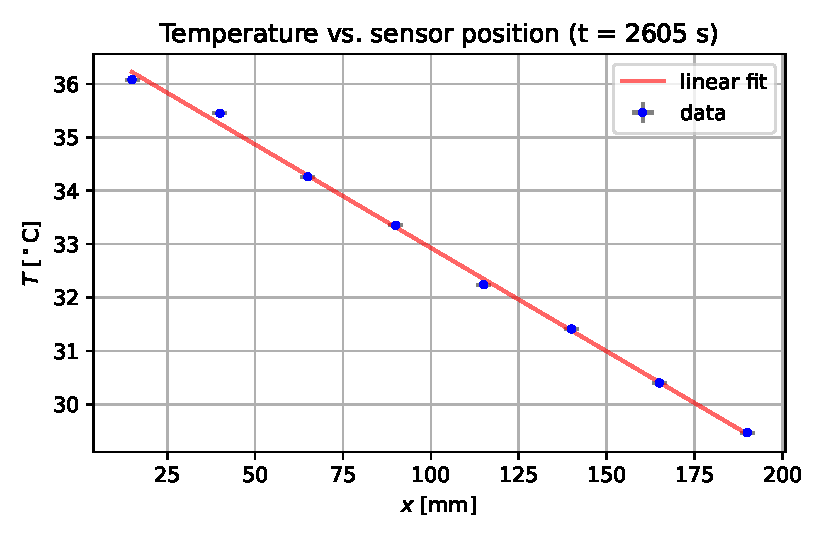
\includegraphics[width=\textwidth]{figures/b_fit_mid.pdf}
    \caption{הטמפרטורה $T$ במעלות צלזיוס כתלות במיקום החיישן $x$ במילימטרים, במדידה שבזמן $t = \BMidTime\U{s}$, וההתאמה הלינארית לפי נוסחה~\eqref{eq:fitb}.}
    \label{fig:b-fit-mid}
  \end{minipage}\hfill
  \begin{minipage}[t]{0.48\textwidth}
    \centering
    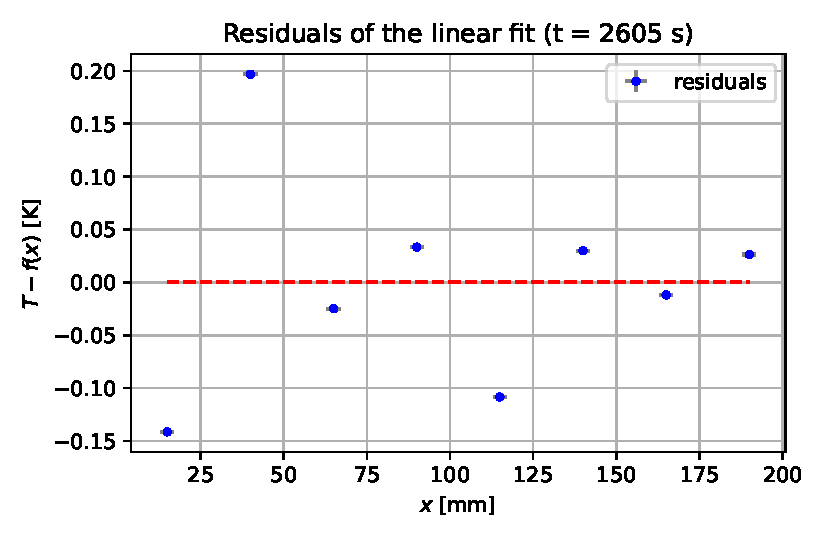
\includegraphics[width=\textwidth]{figures/b_res_mid.pdf}
    \caption{גרף השארים של ההתאמה במדידה שבזמן $t = \BMidTime\U{s}$, בקלווין, כתלות ב-$x$ במילימטרים. צלבי השגיאה מציגים את $\Delta T$ ו-$\Delta x$ בלבד.}
    \label{fig:b-res-mid}
  \end{minipage}
\end{figure}
\begin{figure}[H]
  \centering
  \begin{minipage}[t]{0.48\textwidth}
    \centering
    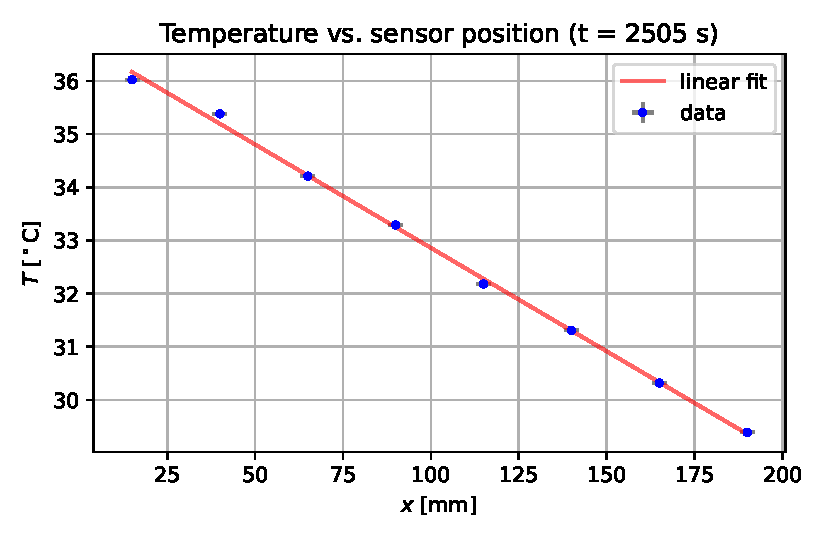
\includegraphics[width=\textwidth]{figures/b_fit_early.pdf}
    \caption{הטמפרטורה $T$ במעלות צלזיוס כתלות במיקום החיישן $x$ במילימטרים, במדידה שבזמן $t = \BEarlyTime\U{s}$, וההתאמה הלינארית לפי נוסחה~\eqref{eq:fitb}.}
    \label{fig:b-fit-early}
  \end{minipage}\hfill
  \begin{minipage}[t]{0.48\textwidth}
    \centering
    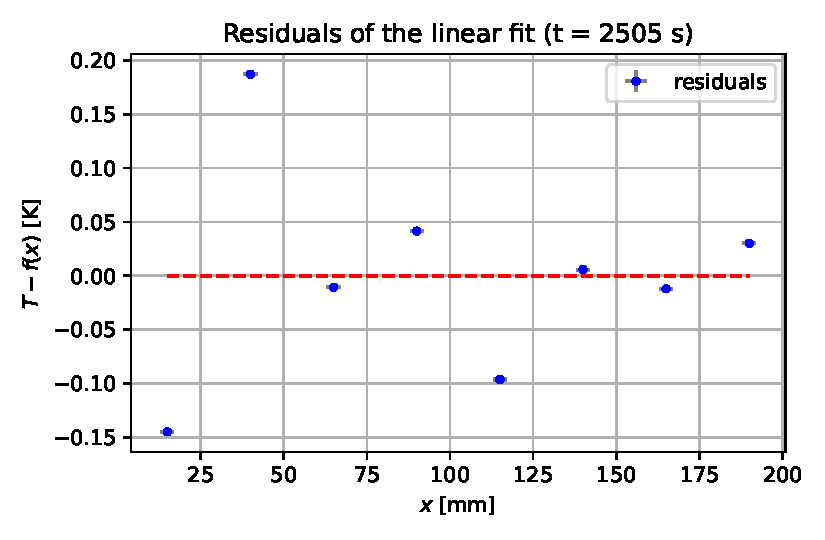
\includegraphics[width=\textwidth]{figures/b_res_early.pdf}
    \caption{גרף השארים של ההתאמה במדידה שבזמן $t = \BEarlyTime\U{s}$, בקלווין, כתלות ב-$x$ במילימטרים. צלבי השגיאה מציגים את $\Delta T$ ו-$\Delta x$ בלבד.}
    \label{fig:b-res-early}
  \end{minipage}
\end{figure}

\subsection*{נספח ג׳ -- הטמפרטורות בהתאמות של חלק ב׳}
% Generated by analysis/analysis.py from the part-b log -- do not edit by hand.
\begin{table}[H]
  \centering
  \renewcommand{\arraystretch}{1.2}
  \begin{tabular}{|c|c|c|c|}
    \hline
    $x\ [\mathrm{mm}]$ & $T(t = 2505\U{s})\ [^\circ\mathrm{C}]$ & $T(t = 2605\U{s})\ [^\circ\mathrm{C}]$ & $T(t = 2705\U{s})\ [^\circ\mathrm{C}]$ \\ \hline
    15 & 36.02 & 36.08 & 36.10 \\ \hline
    40 & 35.38 & 35.45 & 35.47 \\ \hline
    65 & 34.21 & 34.26 & 34.29 \\ \hline
    90 & 33.29 & 33.35 & 33.39 \\ \hline
    115 & 32.18 & 32.24 & 32.29 \\ \hline
    140 & 31.31 & 31.41 & 31.43 \\ \hline
    165 & 30.32 & 30.40 & 30.43 \\ \hline
    190 & 29.39 & 29.47 & 29.50 \\ \hline
  \end{tabular}
  \caption{הטמפרטורות שמדדו שמונת החיישנים בשלוש המדידות של חלק ב׳ שעליהן נעשו ההתאמות, כפי שתועדו בתוכנת ההקלטה. $t$ נמדד מתחילת ההקלטה.}
  \label{tab:raw-b}
\end{table}


\subsection*{נספח ד׳ -- הטמפרטורות בהתאמות של חלק ג׳}
% Generated by analysis/analysis.py from the part-b/c logs -- do not edit by hand.
\begin{table}[H]
  \centering
  \scriptsize
  \renewcommand{\arraystretch}{1.0}
  \setlength{\tabcolsep}{4pt}
  \begin{tabular}{|cc|cc|cc|cc|}
    \hline
    $t\ [\mathrm{s}]$ & $T\ [^\circ\mathrm{C}]$ & $t\ [\mathrm{s}]$ & $T\ [^\circ\mathrm{C}]$ & $t\ [\mathrm{s}]$ & $T\ [^\circ\mathrm{C}]$ & $t\ [\mathrm{s}]$ & $T\ [^\circ\mathrm{C}]$ \\ \hline
    0.000 & 32.50 & 224.976 & 31.91 & 449.932 & 31.38 & 674.898 & 30.86 \\
    4.998 & 32.50 & 229.966 & 31.91 & 454.932 & 31.34 & 679.899 & 30.84 \\
    9.998 & 32.49 & 234.965 & 31.88 & 459.931 & 31.36 & 684.898 & 30.84 \\
    14.997 & 32.47 & 239.963 & 31.90 & 464.930 & 31.34 & 689.897 & 30.84 \\
    19.997 & 32.48 & 244.963 & 31.87 & 469.929 & 31.33 & 694.900 & 30.82 \\
    24.996 & 32.46 & 249.962 & 31.86 & 474.929 & 31.31 & 699.895 & 30.81 \\
    29.995 & 32.46 & 254.962 & 31.84 & 479.928 & 31.31 & 704.895 & 30.78 \\
    34.994 & 32.43 & 259.961 & 31.83 & 484.927 & 31.29 & 709.893 & 30.78 \\
    39.993 & 32.43 & 264.960 & 31.82 & 489.932 & 31.28 & 714.894 & 30.76 \\
    44.993 & 32.39 & 269.959 & 31.81 & 494.926 & 31.27 & 719.893 & 30.76 \\
    49.992 & 32.38 & 274.959 & 31.80 & 499.925 & 31.26 & 724.892 & 30.74 \\
    54.992 & 32.36 & 279.958 & 31.78 & 504.924 & 31.26 & 729.893 & 30.75 \\
    59.990 & 32.34 & 284.958 & 31.78 & 509.924 & 31.23 & 734.890 & 30.72 \\
    64.990 & 32.35 & 289.957 & 31.77 & 514.923 & 31.22 & 739.889 & 30.73 \\
    69.989 & 32.33 & 294.955 & 31.74 & 519.922 & 31.22 & 744.890 & 30.70 \\
    74.998 & 32.30 & 299.955 & 31.72 & 524.921 & 31.20 & 749.888 & 30.69 \\
    79.987 & 32.30 & 304.954 & 31.72 & 529.921 & 31.19 & 754.887 & 30.68 \\
    84.987 & 32.27 & 309.953 & 31.73 & 534.920 & 31.18 & 759.886 & 30.67 \\
    89.985 & 32.27 & 314.953 & 31.69 & 539.919 & 31.18 & 764.885 & 30.67 \\
    94.985 & 32.23 & 319.952 & 31.67 & 544.919 & 31.15 & 769.885 & 30.66 \\
    99.985 & 32.22 & 324.951 & 31.67 & 549.918 & 31.14 & 774.884 & 30.63 \\
    104.984 & 32.23 & 329.950 & 31.67 & 554.917 & 31.13 & 779.884 & 30.64 \\
    109.983 & 32.21 & 334.950 & 31.64 & 559.916 & 31.13 & 784.882 & 30.61 \\
    114.982 & 32.21 & 339.949 & 31.62 & 564.916 & 31.10 & 789.882 & 30.61 \\
    119.982 & 32.21 & 344.948 & 31.61 & 569.915 & 31.10 & 794.881 & 30.60 \\
    124.981 & 32.18 & 349.947 & 31.62 & 574.914 & 31.09 & 799.880 & 30.60 \\
    129.980 & 32.15 & 354.948 & 31.59 & 579.914 & 31.06 & 804.880 & 30.57 \\
    134.979 & 32.16 & 359.946 & 31.59 & 584.912 & 31.06 & 809.879 & 30.57 \\
    139.979 & 32.13 & 364.945 & 31.58 & 589.911 & 31.05 & 814.878 & 30.54 \\
    144.978 & 32.11 & 369.945 & 31.56 & 594.911 & 31.04 & 819.878 & 30.55 \\
    149.977 & 32.11 & 374.944 & 31.54 & 599.911 & 31.04 & 824.877 & 30.54 \\
    154.976 & 32.09 & 379.943 & 31.54 & 604.909 & 31.01 & 829.876 & 30.52 \\
    159.976 & 32.08 & 384.949 & 31.53 & 609.909 & 31.02 & 834.875 & 30.51 \\
    164.975 & 32.08 & 389.941 & 31.52 & 614.908 & 30.99 & 839.875 & 30.51 \\
    169.974 & 32.06 & 394.941 & 31.52 & 619.907 & 30.99 & 844.874 & 30.50 \\
    174.974 & 32.04 & 399.939 & 31.50 & 624.916 & 30.95 & 849.873 & 30.49 \\
    179.973 & 32.03 & 404.939 & 31.48 & 629.906 & 30.97 & 854.872 & 30.47 \\
    184.973 & 32.03 & 409.938 & 31.47 & 634.905 & 30.95 & 859.871 & 30.46 \\
    189.971 & 32.01 & 414.938 & 31.45 & 639.905 & 30.94 & 864.870 & 30.45 \\
    194.971 & 31.99 & 419.946 & 31.45 & 644.903 & 30.92 & 869.870 & 30.44 \\
    199.970 & 32.00 & 424.936 & 31.44 & 649.903 & 30.92 & 874.869 & 30.42 \\
    204.968 & 31.97 & 429.936 & 31.43 & 654.902 & 30.90 & 879.868 & 30.42 \\
    209.969 & 31.97 & 434.934 & 31.41 & 659.902 & 30.91 & 884.868 & 30.41 \\
    214.968 & 31.96 & 439.934 & 31.40 & 664.900 & 30.88 & 889.867 & 30.40 \\
    219.967 & 31.94 & 444.933 & 31.40 & 669.900 & 30.87 & 894.866 & 30.38 \\
    \hline
  \end{tabular}
  \caption{\relax{הטמפרטורה שמדד חיישן 4 במקטע הקירור, 180 מדידות, כפי שתועדו בתוכנת ההקלטה. $t$ נמדד מתחילת ההקלטה בחלק ג׳.}}
  \label{tab:raw-c-cool}
\end{table}
\begin{table}[H]
  \centering
  \scriptsize
  \renewcommand{\arraystretch}{1.0}
  \setlength{\tabcolsep}{4pt}
  \begin{tabular}{|cc|cc|cc|cc|}
    \hline
    $t\ [\mathrm{s}]$ & $T\ [^\circ\mathrm{C}]$ & $t\ [\mathrm{s}]$ & $T\ [^\circ\mathrm{C}]$ & $t\ [\mathrm{s}]$ & $T\ [^\circ\mathrm{C}]$ & $t\ [\mathrm{s}]$ & $T\ [^\circ\mathrm{C}]$ \\ \hline
    1084.838 & 34.00 & 1219.818 & 36.61 & 1354.798 & 39.10 & 1489.778 & 41.51 \\
    1089.838 & 34.09 & 1224.817 & 36.71 & 1359.797 & 39.20 & 1494.776 & 41.59 \\
    1094.837 & 34.19 & 1229.817 & 36.80 & 1364.796 & 39.29 & 1499.776 & 41.68 \\
    1099.836 & 34.29 & 1234.816 & 36.89 & 1369.795 & 39.40 & 1504.776 & 41.76 \\
    1104.835 & 34.39 & 1239.815 & 37.00 & 1374.795 & 39.46 & 1509.775 & 41.85 \\
    1109.842 & 34.50 & 1244.814 & 37.08 & 1379.794 & 39.57 & 1514.774 & 41.93 \\
    1114.834 & 34.58 & 1249.813 & 37.19 & 1384.794 & 39.65 & 1519.773 & 42.02 \\
    1119.834 & 34.69 & 1254.813 & 37.26 & 1389.793 & 39.75 & 1524.773 & 42.11 \\
    1124.831 & 34.79 & 1259.812 & 37.37 & 1394.792 & 39.82 & 1529.771 & 42.20 \\
    1129.831 & 34.88 & 1264.812 & 37.45 & 1399.791 & 39.92 & 1534.771 & 42.26 \\
    1134.831 & 34.98 & 1269.811 & 37.53 & 1404.790 & 39.99 & 1539.771 & 42.36 \\
    1139.830 & 35.07 & 1274.809 & 37.65 & 1409.789 & 40.10 & 1544.770 & 42.43 \\
    1144.829 & 35.16 & 1279.809 & 37.74 & 1414.789 & 40.19 & 1549.769 & 42.53 \\
    1149.828 & 35.25 & 1284.809 & 37.83 & 1419.788 & 40.28 & 1554.768 & 42.62 \\
    1154.828 & 35.36 & 1289.808 & 37.91 & 1424.787 & 40.36 & 1559.767 & 42.70 \\
    1159.826 & 35.47 & 1294.814 & 38.01 & 1429.787 & 40.46 & 1564.766 & 42.78 \\
    1164.826 & 35.55 & 1299.806 & 38.10 & 1434.786 & 40.55 & 1569.766 & 42.86 \\
    1169.826 & 35.66 & 1304.806 & 38.19 & 1439.785 & 40.64 & 1574.765 & 42.95 \\
    1174.825 & 35.75 & 1309.804 & 38.29 & 1444.786 & 40.74 & 1579.764 & 43.04 \\
    1179.824 & 35.86 & 1314.804 & 38.39 & 1449.784 & 40.83 & 1584.764 & 43.12 \\
    1184.823 & 35.95 & 1319.803 & 38.47 & 1454.783 & 40.89 & 1589.763 & 43.20 \\
    1189.822 & 36.06 & 1324.802 & 38.57 & 1459.782 & 40.99 & 1594.762 & 43.28 \\
    1194.821 & 36.13 & 1329.802 & 38.64 & 1464.781 & 41.07 & 1599.762 & 43.36 \\
    1199.821 & 36.22 & 1334.801 & 38.76 & 1469.781 & 41.16 & 1604.761 & 43.44 \\
    1204.820 & 36.32 & 1339.799 & 38.84 & 1474.780 & 41.25 & 1609.760 & 43.53 \\
    1209.819 & 36.43 & 1344.802 & 38.93 & 1479.779 & 41.33 & 1614.759 & 43.62 \\
    1214.819 & 36.52 & 1349.799 & 39.02 & 1484.779 & 41.40 & 1619.759 & 43.69 \\
    \hline
  \end{tabular}
  \caption{\relax{הטמפרטורה שמדד חיישן 4 במקטע החימום (הדקות 3--12 לאחר הפעלת ספק הכוח), 108 מדידות, כפי שתועדו בתוכנת ההקלטה. $t$ נמדד מתחילת ההקלטה בחלק ג׳.}}
  \label{tab:raw-c-heat}
\end{table}
\begin{table}[H]
  \centering
  \scriptsize
  \renewcommand{\arraystretch}{1.0}
  \setlength{\tabcolsep}{4pt}
  \begin{tabular}{|cc|cc|cc|cc|}
    \hline
    $t\ [\mathrm{s}]$ & $T\ [^\circ\mathrm{C}]$ & $t\ [\mathrm{s}]$ & $T\ [^\circ\mathrm{C}]$ & $t\ [\mathrm{s}]$ & $T\ [^\circ\mathrm{C}]$ & $t\ [\mathrm{s}]$ & $T\ [^\circ\mathrm{C}]$ \\ \hline
    2504.627 & 33.29 & 2559.618 & 33.32 & 2614.610 & 33.36 & 2669.603 & 33.37 \\
    2509.626 & 33.31 & 2564.617 & 33.33 & 2619.609 & 33.35 & 2674.602 & 33.36 \\
    2514.626 & 33.30 & 2569.617 & 33.32 & 2624.609 & 33.36 & 2679.601 & 33.36 \\
    2519.625 & 33.29 & 2574.616 & 33.33 & 2629.608 & 33.35 & 2684.599 & 33.37 \\
    2524.624 & 33.29 & 2579.615 & 33.33 & 2634.609 & 33.36 & 2689.599 & 33.37 \\
    2529.623 & 33.28 & 2584.615 & 33.35 & 2639.607 & 33.35 & 2694.599 & 33.37 \\
    2534.622 & 33.30 & 2589.614 & 33.33 & 2644.605 & 33.36 & 2699.598 & 33.39 \\
    2539.621 & 33.30 & 2594.613 & 33.34 & 2649.605 & 33.37 & 2704.597 & 33.39 \\
    2544.621 & 33.31 & 2599.613 & 33.34 & 2654.605 & 33.35 &  &  \\
    2549.620 & 33.31 & 2604.612 & 33.35 & 2659.603 & 33.36 &  &  \\
    2554.620 & 33.33 & 2609.611 & 33.35 & 2664.603 & 33.35 &  &  \\
    \hline
  \end{tabular}
  \caption{\relax{הטמפרטורה שמדד חיישן 4 ב-200 השניות האחרונות של ההקלטה בחלק ב׳, 41 מדידות, כפי שתועדו בתוכנת ההקלטה. $t$ נמדד מתחילת ההקלטה בחלק ב׳.}}
  \label{tab:raw-c-exp}
\end{table}


\end{document}
